%************************************************
\chapter{Model evaluation in the Southern Ocean} % $\mathbb{ZNR}$
%************************************************

\label{ch:eval}

%\paragraph{Flow of section - maybe belongs to Introduction last paragraph}
%The Southern Ocean is located on the Southern hemisphere around the Antarctic continent. As the atmospheric waves are disturbed by only few land masses, the Southern ocean carries very zonally symmetric features.

%The variations of oceanic carbon uptake are related to the dynamic background changes in ocean circulation and possibly biology \citep{LeQuere2007}. 
My analysis of the internal variability of the Southern Ocean carbon sink originates in the evaluation of air-sea CO$_2$ flux (\autoref{sec:co2flux_model_eval}). As the strength of the CO$_2$ flux in the Southern Ocean is modulated by the strength of westerly winds \citep{Lovenduski2007}, I assess also the sea-level pressure fields (\autoref{sec:winds_model_eval}) as well as biology (\autoref{sec:biology}) and upper-ocean circulation, which respond to changes in wind (\autoref{sec:UOOC}).

A previous model evaluation of \acs{HAMOCC} for the \ac{CMIP5} provides a global view on biogeochemistry \citep{Ilyina2013}. In this chapter I evaluate the model focusing on the Southern Ocean and specifically the processes related to the carbon sink. In each subsection I compare the modeled mean state of the Southern Ocean to observational data and assess modeled decadal internal variability in spatial distribution and temporal evolution. 


 

\section{CO$_2$ flux}
\label{sec:co2flux_model_eval}

%intro paragraph on CO2flux drivers
The patterns of CO$_2$ flux are mainly controlled by primary production (see in detail \autoref{sec:biology}) and advective transport of \acs{DIC} and alkalinity (see in detail \autoref{sec:UOOC}). Ekman suction, also referred to as upwelling, drives outgassing and Ekman subduction, also referred to as downwelling, drives CO$_2$ uptake or ingassing. Positive values in sea-air CO$_2$ flux indicate outgassing and negative values CO$_2$ uptake by the oceans.\newline %kick because in figure caption?

%\paragraph{Spatial distribution in mean state} 
The climatological ensemble mean state from 1980 to 2004 of the Southern Ocean CO$_2$ flux in \acs{MPI-ESM} marks the Antarctic coastal region is a CO$_2$ sink, whereas the upwelling waters in the Atlantic and Indian sector at 50-60$^\circ$S are outgassing regions and CO$_2$ flux neutral in the Pacific (\autoref{fig:SOCS_ensmean_ensstd-a}). North of 50$^\circ$S, the oceans take up CO$_2$ because of stronger primary production and Ekman subduction.\newline

%The Southern Ocean is - next to coastal regions - the main area for upwelling from deep waters. These carbon-rich waters equilibrate with at the surface with the atmosphere. For this process of outgassing, I use positive values of CO$_2$ flux. Outgassing from upwelling waters predominantly happens at 50-60$^\circ$S in the atlantic and indian ocean sector (fig. \autoref{fig:SOCS_ensmean_ensstd}a). Further north relatively saline Antartic Intermediate Waters (AAIW) get subducted under warmer subtropical waters. This process of downwelling transports anthropogenic carbon into the ocean interior and hence is a carbon uptake region. Near to the Antarctic continent south of 60$^\circ$S, brine injections and surface cooling drives the sinking of waters via open ocean convection, but at the same time sea-ice hinders CO$_2$ flux. 
 
%\paragraph{Spatial mean comparison to observational data}
The observational-based estimate \acs{SOM-FFN} shows similar patterns of carbon uptake and outgassing but in lower absolute values (\autoref{fig:SOCS_ensmean_ensstd-c}). 
Hardly any measurements in the region of seasonal ice cover make a comparison with observation-based values hard to interpret.\newline
%This model evaluation of CO$_2$ flux is very similar to the related comparison of pCO$_2$ with \citep{Takahashi2009}.
%The modeled pCO$_2$ is very similar to the results in \citep{Ilyina2013}.

%\paragraph{Spatial distribution of internal variability} 
For spatial distributions I define decadal internal variability $\sigma_{DIV}$ as the standard deviation over the changes in decades in the whole ensemble (\autoref{sec:DIV}).

The region 45-60$^\circ$S is most variable and characterized by upwelling (\autoref{fig:UOOC_mean-a}) and the southern edge of primary production (\autoref{fig:SO_intpp_ensmean_ensstd-a}). The change in latitudinal position and strength of the westerly winds affects the position and amplitude of upwelling (\autoref{sec:UOOC}) and primary production (\autoref{sec:biology}).\newline

%\paragraph{Spatial variability comparison to observational data}
The observation-based \acs{SOM-FFN} decadal variability $\sigma_{DIV}$ is most pronounced at 50-60$^\circ$S in the Atlantic and Indian and south of 60$^\circ$S in the Pacific \citep{Landschuetzer2016}. The amplitude of decadal variability is smaller than in \acs{MPI-ESM} (\autoref{fig:SOCS_ensmean_ensstd-d}). However, this comparison is limited by large differences in sample size between the 22-year observational record and the 100 \acs{MPI-ESM} realizations.\newline %how relevant is this plot? 
%Reference to CMIP5 mean and std [later in appendix]?



\def\stackalignment{l}



\begin{figure}[bth]
        %\myfloatalign
        \subfloat[\acs{MPI-ESM} ensemble mean CO$_2$ flux \text{      } \text{[kgC m$^{-2}$yr$^{-1}$ /8yrs]}]
        {\label{fig:SOCS_ensmean_ensstd-a}%
       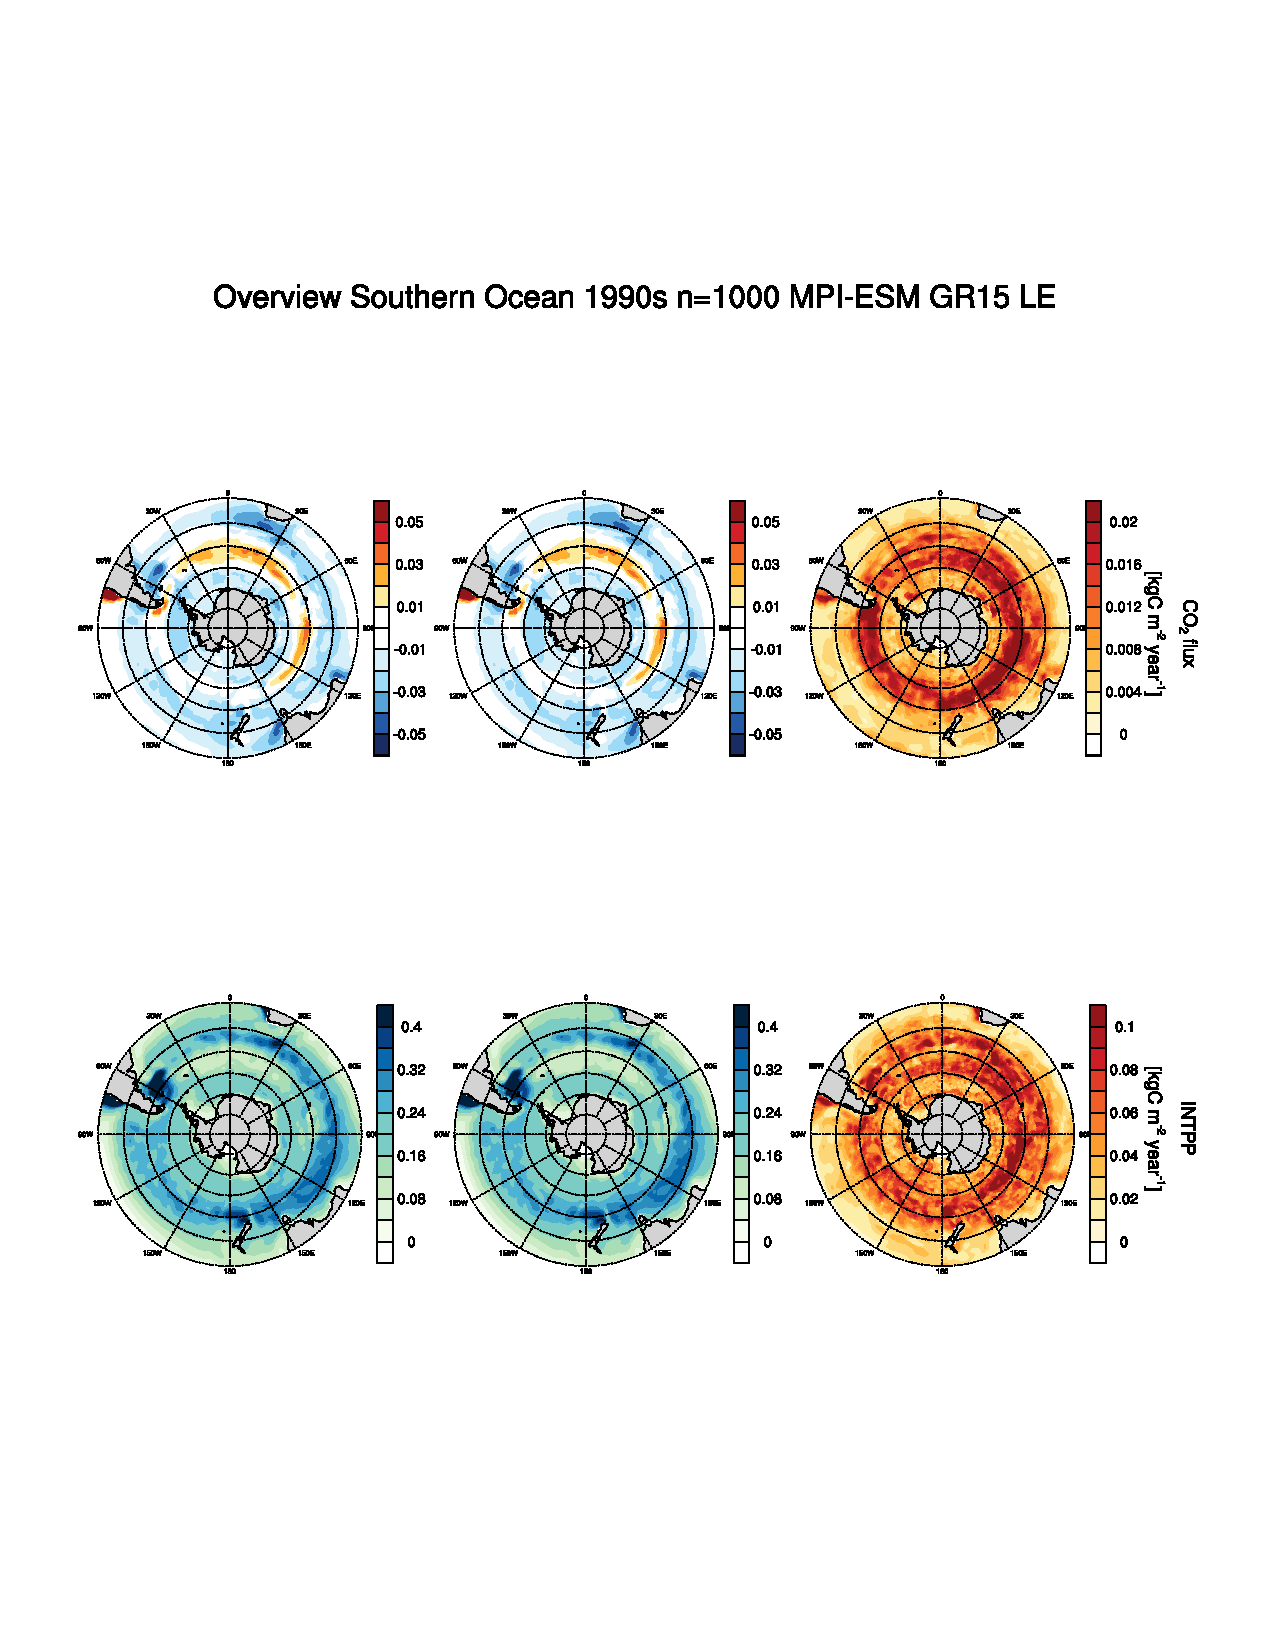
\includegraphics[scale=.95,page=1,trim=7.25cm 15cm 8.2cm 8.4cm,clip]{Overview_SO_co2flux_intpp_ens_t1990s.pdf}} %\quad
       \subfloat[\acs{MPI-ESM} $\sigma_{DIV}$ CO$_2$ flux  \text{      }  \text{      } \text{[kgC m$^{-2}$yr$^{-1}$ /8yrs]}]
        {\label{fig:SOCS_ensmean_ensstd-b}%
       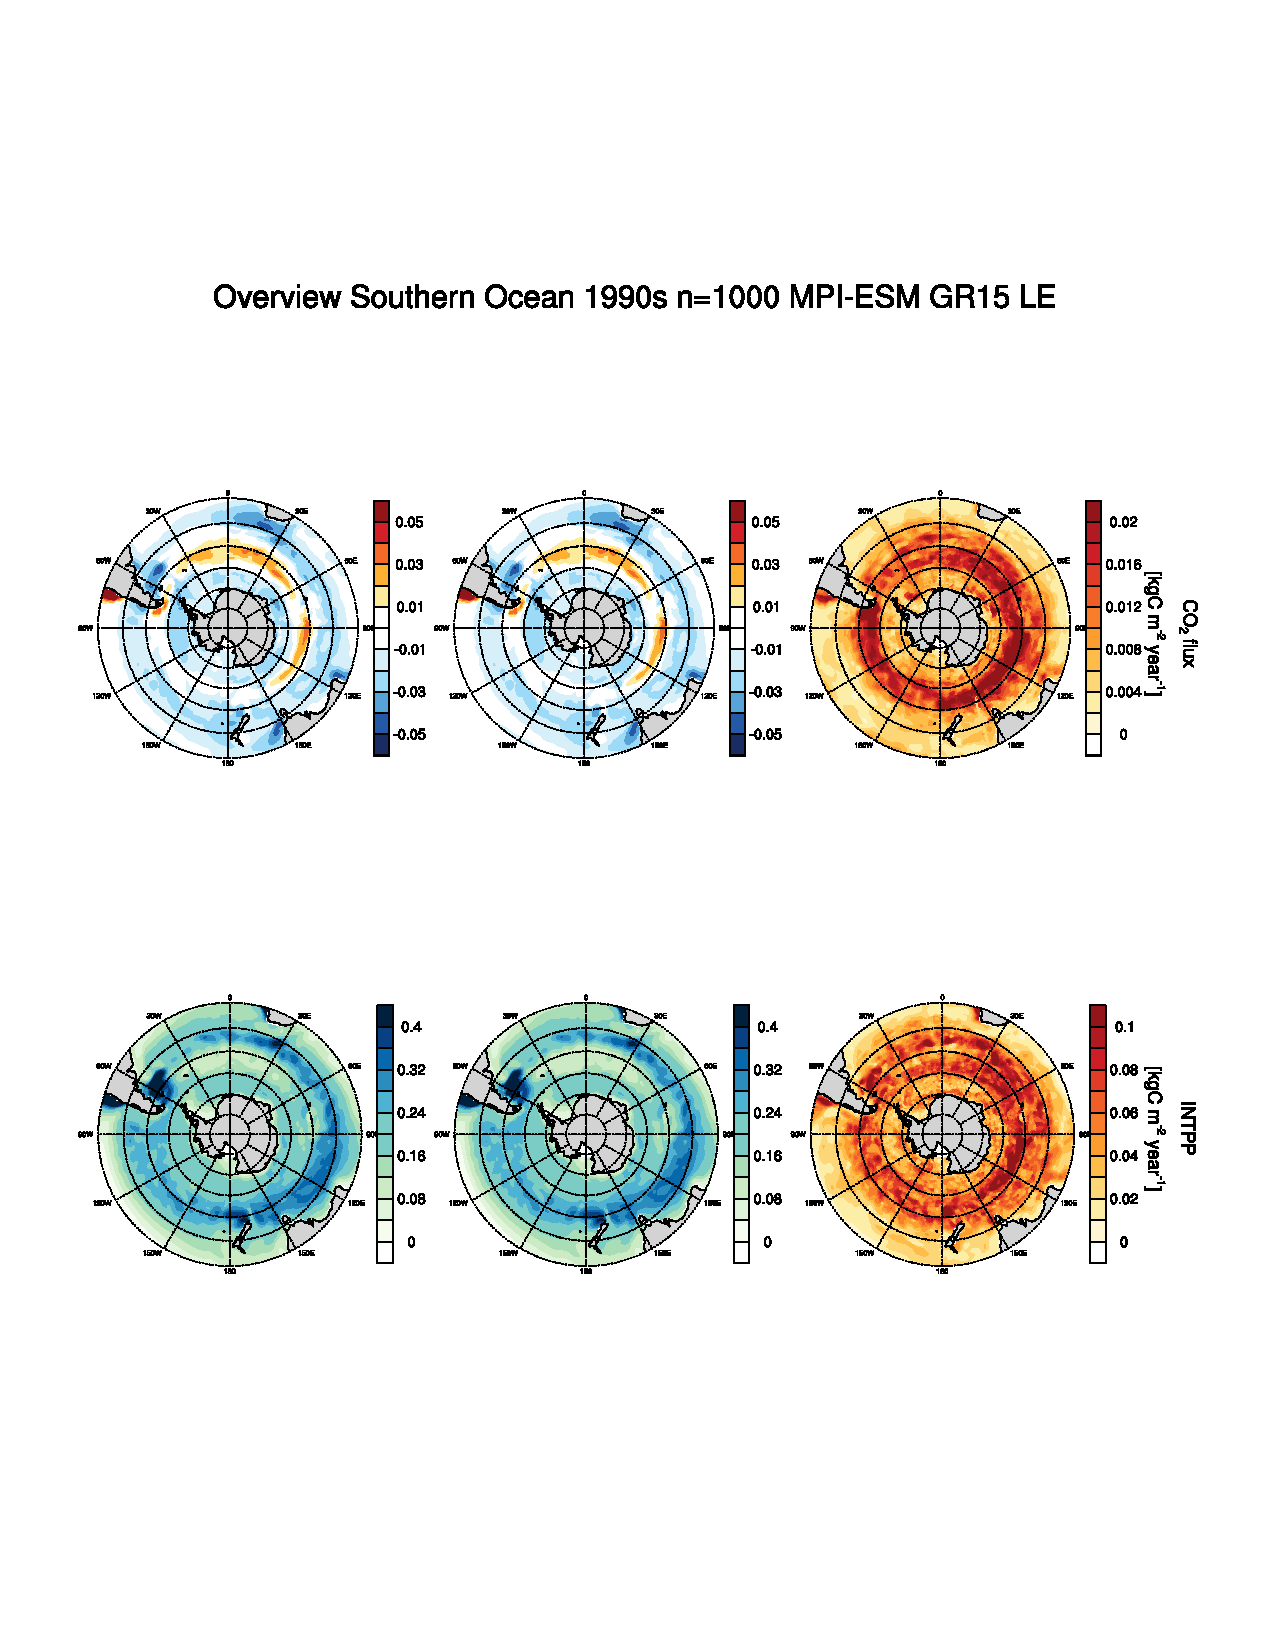
\includegraphics[scale=.95,page=1,trim=13.4cm 15cm 2.25cm 8.4cm,clip]{Overview_SO_co2flux_intpp_ens_t1990s.pdf}} \\
       
        \subfloat[\acs{SOM-FFN} mean CO$_2$ flux \text{      }  \text{      } \text{[kgC m$^{-2}$yr$^{-1}$ /8yrs]}]
        {\label{fig:SOCS_ensmean_ensstd-c}%
         \includegraphics[scale=.95,page=2,trim=7.25cm 15cm 8.2cm 8.4cm,clip]{Overview_SO_co2flux_intpp_ens_t1990s.pdf}} 
        \subfloat[\acs{SOM-FFN} $\sigma_{DIV}$ CO$_2$ flux \text{      }  \text{      } \text{[kgC m$^{-2}$yr$^{-1}$ /8yrs]}]
        {\label{fig:SOCS_ensmean_ensstd-d}%
         \includegraphics[scale=.95,page=2,trim=13.4cm 15cm 2.25cm 8.4cm,clip]{Overview_SO_co2flux_intpp_ens_t1990s.pdf}} 
        \caption{Spatial distribution of the climatology (a,c) and decadal internal variability $\sigma_{DIV}$ (b,d) from 1980-2004 of the Southern Ocean sea-air CO$_2$ flux: (a) \acs{MPI-ESM LE} ensemble mean as forced signal, (b) ensemble decadal standard deviation as decadal internal variability $\sigma_{DIV}$, (c) \acs{SOM-FFN} climatology 1982-2004, (d) \acs{SOM-FFN} decadal variability $\sigma_{DIV}$; negative values indicate ocean uptake.} \label{fig:SOCS_ensmean_ensstd}
\end{figure}

\clearpage
\begin{figure}[hbt]
        \myfloatalign
        \captionsetup[subfigure]{labelformat=empty,justification=centering}
        \subfloat[Annual sea-Air CO$_2$ flux anomaly \text{[PgC/yr]}]
        {\includegraphics[scale=.48,angle=90,page=2,trim=4cm 1.2cm 4.5cm 2.5cm,clip]{co2flux_SO_timeseries_ymjm_35S_1980_2015_trend_8}} 
        \caption{Temporal evolution of the Southern Ocean sea-air CO$_2$ flux anomaly south of 35$^\circ$S with respect to the 1980s. Grey lines show the 100 ensemble members, the black line the ensemble mean, the blue shading is the ensemble decadal internal variability $\sigma_{DIV}$, the red line shows the most  positive 8-year trend, the blue line shows the most negative 8-year trend, the green line represents the \acs{SOM-FFN} observation-based estimate \citep{landschuetzer2015}; negative values indicate carbon uptake; \acs{MPI-ESM LE} is extended under \acs{RCP}4.5 forcing from 2005 to 2015.}\label{fig:evolution_southern_ocean_carbon_sink}
\end{figure}

%\paragraph{Temporal evolution of the mean state and internal variability}
The temporal evolution of the Southern Ocean ensemble mean CO$_2$ flux south of 35$^\circ$S is dominated by the forced negative trend of rising atmospheric CO$_2$ concentrations (\autoref{fig:evolution_southern_ocean_carbon_sink}). Still, no individual realization follows the negative trend strictly monotonic - they oscillate around the ensemble mean state triggered by internal variability. Exemplary, the most extreme monotonic positive and negative 8-year trend is highlighted. The modeled ensemble mean sea-air CO$_2$ flux over the historical period 1980-2004 is $\sim-1.15$ PgC/yr and decadal internal variability $\sigma_{DIV}$ is $\sim\pm0.19$ PgC/yr/decade, larger than the forced signal of $\sim-0.14$ PgC/yr/decade, which reflects the mean of decadal changes. {\color{RoyalBlue}Tab.} \ref{tab:trends_co2flux} shows an overview the statistical quantities related to Southern Ocean carbon sink variability.\newline

%\paragraph{Temporal comparison to observational data} 
The observational-based estimate for the whole region south of 35$^\circ$S shows a strong positive CO$_2$ flux trend in the 1990s and a strong negative trend reinvigorating the carbon sink in the 2000s \citep{landschuetzer2015} (\autoref{fig:evolution_southern_ocean_carbon_sink}). The modeled $\sigma_{DIV}$ is lower than of decadal variations in \acs{SOM-FFN} (\autoref{tab:trends_co2flux}). This means that on multi-year time-scales \acs{SOM-FFN} is 50\% more variable than \acs{MPI-ESM LE}. This comparison must be ingested with caution as influent datasets differ in ensemble-space. \acs{SOM-FFN} would rank as one exceptionally variable 22-year realization into \acs{MPI-ESM LE}.\newline

\begin{table}[hbt]
%\centering
\small
\begin{tabular}{lcccc}
\multicolumn{5}{l} {trend length [TL]} \hspace{.1cm} {8-yr trend} \hspace{1.4cm} {10-yr trend} \hspace{1.cm} \\ \hline
%{8-yr trend} \multicolumn{2}{l} 50-60$^\circ$S \multicolumn{2}{l} 40-50$^\circ$S} \\ \hline
  dataset & \footnotesize \acs{MPI-ESM}  & \footnotesize\acs{SOM-FFN} & \footnotesize\acs{MPI-ESM}  &\footnotesize \acs{SOM-FFN}  \\
  \hline
  mean state [PgC/yr]					& -1.15 & -0.87 & -1.15 & -0.87 \\
  $\sigma_{DIV}$ [PgC/yr/TL]			& $\pm$0.22 & $\pm$0.35 & $\pm$0.19 & $\pm$0.30 \\
  forced signal [PgC/yr/TL] 			& -0.11 & / & -0.14 & / \\
  \hline \hline
  positive trend [PgC/yr/TL]			& +0.70 & +0.38 & +0.53 & +0.39 \\
  corrected trend [PgC/yr/TL]			& +0.81 & +0.49 & +0.67 & +0.53 \\
  probability [\%]						& 0.01  &	20	&  0.1	&	10	\\
  \hline
  negative trend [PgC/yr/TL]			& -0.78 & -0.53 & -0.74 & -0.66 \\
  corrected trend [PgC/yr/TL]			& -0.67 & -0.39 & -0.60 & -0.52 \\
  probability [\%]						&  0.3	&	25	&	0.3	&	10	
\end{tabular}
\caption{Overview of statistical quantities in two trend lengths [TL] in sea-air CO$_2$ flux in the Southern Ocean south of 35$^\circ$S from \acf{MPI-ESM LE} and \acf{SOM-FFN} \citep{landschuetzer2015}; positive and negative trends are the most extreme trends in each dataset; the forced signal is subtracted off the corrected trends; probabilities quantify the likelihood that corrected trends are due to internal variability; 8-yr trends are required to be monotonic.}
\label{tab:trends_co2flux}
\end{table}


The decadal variability $\sigma_{DIV}$ in \acs{SOM-FFN} data is $\sim0.30$ PgC/yr/ decade, with the most positive CO$_2$ flux trend in the 1990s of $\sim+0.39$ PgC/yr/decade and the most negative trend of $\sim-0.66$ PgC/yr/ decade. Compared to \acs{SOM-FFN}'s $\sigma_{DIV}$, both observation-based trends corrected for the modeled forced signal get an attribution to internal variability of $\sim10$\% ($\sim1.6\sigma$). Under the context of \acs{MPI-ESM LE}'s $\sigma_{DIV}$ these magnitudes in observation-based trends could be due to internal variability with probabilities of 1\% ($\sim2.6\sigma$) for 1990s and 2000s trends respectively. This outlines the low likelihood of these \acs{SOM-FFN} CO$_2$ flux trends attributed to internal variability from the perspective of numerical modeling with perturbed initial conditions (\autoref{tab:trends_co2flux}).

As \acs{MPI-ESM LE} simulations are forced with prescribed atmospheric CO$_2$ concentrations, the modeled internal variability of an interactive carbon cycle would be a more realistic counterpart for the observed internal variability. The non-linear changes in atmospheric CO$_2$ concentrations due to the interplay of the oceanic and terrestrial carbon cycle result in 25\% higher internal variability \citep{Ilyina2013}.\newline



%\paragraph{Choice of trends} 
%To analyze the processes driving this decadal internal variability $\sigma_{DIV}$, I focus on individual ensemble realizations. Here, I have to make a compromise between signal strength and robustness versus trendlength. It is a trade-off between decadal and inter-annual variability. The longer a period, the more likely the trend deviates from a monotonic behavior. Therefore longer trends show a less strong signal per trendlength (Fig. \autoref{fig:heatmap}). Longer trends also experience a stronger influence of atmospheric forced trend. I decided to analyze 8-year trends, because they are still very close to a decade, but still they are able to show similar magnitude and monotonic behavior as the observation-based estimate. 


%\paragraph{Highlighted monotonic CO$_2$ flux trends}
%I select the most extreme positive and negative monotonic trends. 
Applying the selection criteria from \autoref{sec:choicetrend} I focus on the two highlighted extreme CO$_2$ flux trends with monotonic behavior (\autoref{fig:evolution_southern_ocean_carbon_sink}). For decadal 10-year trends the most extreme cases are of the same magnitude ($\sim+0.5$ PgC/yr/decade and $\sim-0.7$ PgC/yr/decade) as those derived from observation-based estimates in the 1990s and 2000s \citep{landschuetzer2015} (\autoref{fig:heatmap}). The processes related to decadal and multi-year trends only differ in monotony. Longer trends are more strongly exposed to the forced trend and likely dominated strong short-term varibility and hence do not persist as long. In the following I always also analyze the drivers of two distinct 8-year trends. The most positive monotonic 8-year air-sea CO$_2$ flux trend from 1985 to 1992 in ensemble 78 reaches $\sim+0.5$ PgC/yr/8yrs and the most negative monotonic 8-year trend from 1995 to 2002 in ensemble 143 reaches $\sim-0.6$ PgC/yr/8yrs. 
%Analyzing a range of trend lengths from 6 to 14 years, I assess that \acs{MPI-ESM LE} is able to capture positive and negative multi-year and decadal CO$_2$ flux trends in the Southern Ocean (\autoref{fig:heatmap}). 

%I choose extreme monotonic trends to study the processes driving internal variability in the carbon cycle because stronger trends will give me a stronger signal in the underlying processes, which are discussed in chapter \autoref{ch:trends}.\newline %Therefore, I choose to analyze 8-year trends which are a compromise between trendlength (supposed to be 10 year for decadal variability) and a clearer signal (decays over time).

%The positive CO$_2$ flux trend highlighted in red is 0.7 PgC/8yrs, the negative CO$_2$ flux trend highlighted in blue is -0.8 PgC/8yrs. Those trends are higher than the corresponding trends in the 1990s and 2000s from SOM-FFN, but they that's also not the point of my study.  


%\paragraph{Comparison of ensemble CO$_2$ flux internal variability} This is in contrast to other perturbed inital conditions large ensembles (see section \autoref{sec:PICLE}). Neither \acs{CESM} \acs{LE} nor \acs{GFDL} \acs{LE} can reproduce similar strong decadal CO$_2$ flux trends in the Southern Ocean [personal communication Nikki Lovenduski, Sarah Schlunegger]. \cite{McKinley2016} mentioned a weak carbon sink for \acs{CESM} \acs{LE}. \cite{Resplandy2015} showed that \acs{MPI-ESM}'s dominant area of internal variability is the Southern Ocean, whereas \acs{CESM} is most variable in the tropical and Indian pacific and \acs{GFDL} has large internal variability in tropical Indian pacific as well as the Southern Ocean.

%The different method of initialization could not have caused the behavior of trends, because the CO$_2$ flux pathways of different realizations already cross after few years and upper ocean loses his history after 50 years. The internal variability specific to the model itself is dominating \citep{Lovenduski2016}.  







\clearpage
\section{Winds}
\label{sec:winds_model_eval}
%\paragraph{Spatial distribution in the mean state}
%The Southern Ocean is located on the Southern hemisphere around the Antarctic continent. As the atmospheric waves are disturbed by only few land masses and the insolation changes latitudinal, the Southern ocean carries very zonally symmetric features.
Winds are governed by distributions in \ac{SLP}. They point from high pressure to low pressure systems, but get diverted to their left in the Southern Hemisphere by the Coriolis force. Therefore, strong westerly winds are established between the low-pressure system south of 45$^\circ$S and higher pressure systems over the subtropical gyres (\autoref{fig:SO_winds_ensmean_ensstd-a}). This zonally symmetric \acs{SLP} pattern in the ensemble climatological mean leads to zonally symmetric westerly winds peaking at 50$^\circ$S.\newline

%\paragraph{Spatial mean comparison to observational data}
The spatial zonal distribution in observational data of a reanalysis climatology from \acf{NCEP} is so similar to the \acs{MPI-ESM LE} climatology that I plot the difference between \acs{MPI-ESM LE} climatology and \acs{NCEP} reanalysis \citep{Kalnay1996} (\autoref{fig:SO_winds_ensmean_ensstd-c}). The position of the jets in \acs{ECHAM} is shifted to lower latitudes \citep{Stevens2013} which seems to be a common atmospheric modeling challenge \citep{Kidston2010}. Therefore, the modeled westerlies are too strong from 30-60$^\circ$S and too weak south of 60$^\circ$S. The zonal wind speed difference peaks at 45$^\circ$S at $+1$m/s.

The decadal internal variability $\sigma_{DIV}$ increases zonally towards lower latitudes with the highest internal decadal variability in the pacific sector in the Southern Ocean seasonal ice-covered area (\autoref{fig:SO_winds_ensmean_ensstd-b}).\newline

%\paragraph{Spatial internal variability comparison to observational data}
Observational reanalysis data reveal the same spatial distribution with a higher amplitude of decadal internal variability (\autoref{fig:SO_winds_ensmean_ensstd-d}). The pacific sector reflects the area of an Antarctic dipole induced from the \ac{ENSO}, which manifests itself in variability of sea-ice \citep{Yuan2004}. This is also known as the Pacific-South American (PSA) Oscillation \citep{Sallee2008}. The atmospheric Southern Ocean jet splits and in El Ni\~{n}o conditions intensifies on a northern route  inducing a low pressure system with more storms. La Ni\~{n}a conditions bring a high pressure system with less storms vice versa. Such tele-connections of the tropics into the Southern Ocean are subject of current research and have been rarely analyzed yet for the Southern Ocean carbon sink.\newline

%The direction of winds is lost in the calculation of standard deviations, therefore the wind arrows in fig. \autoref{fig:SO_winds_ensmean_ensstd}b,d only show the magnitude of the internal variability of winds which is highest in the pacific sector of the Southern Ocean and generally decreases with latitude.

\begin{figure}[hbt]
        %\myfloatalign
        \subfloat[\acs{MPI-ESM LE} mean \acs{SLP} \text{[hPa/8yrs]}]
        {\label{fig:SO_winds_ensmean_ensstd-a}%
       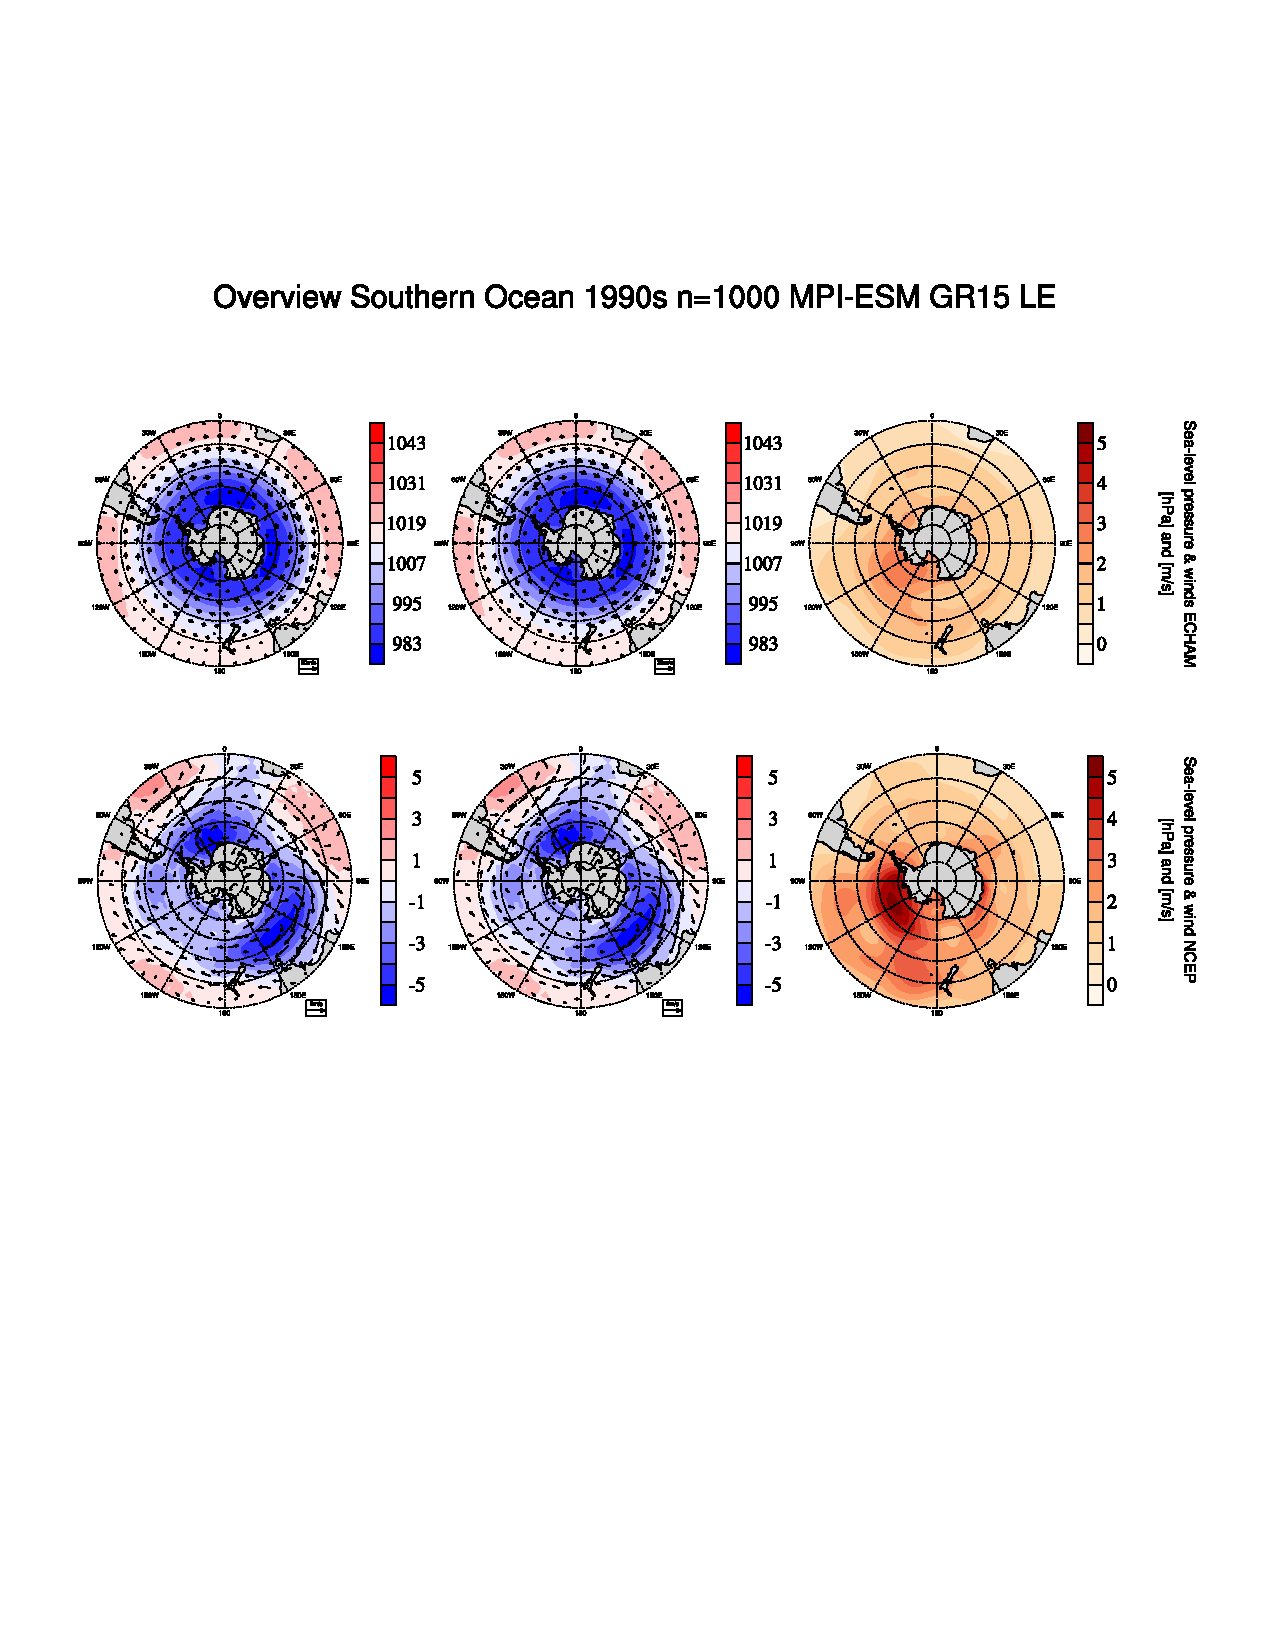
\includegraphics[scale=1,page=1,trim=7.25cm 16.5cm 8.2cm 7cm,clip]{Overview_SO_slp_ens_t1990s.pdf}} %\quad
       \subfloat[\acs{MPI-ESM} \acs{SLP} $\sigma_{DIV}$ \text{[hPa/8yrs]} \text{      }  \text{      } \text{      }  \text{      }]
        {\label{fig:SO_winds_ensmean_ensstd-b}%
       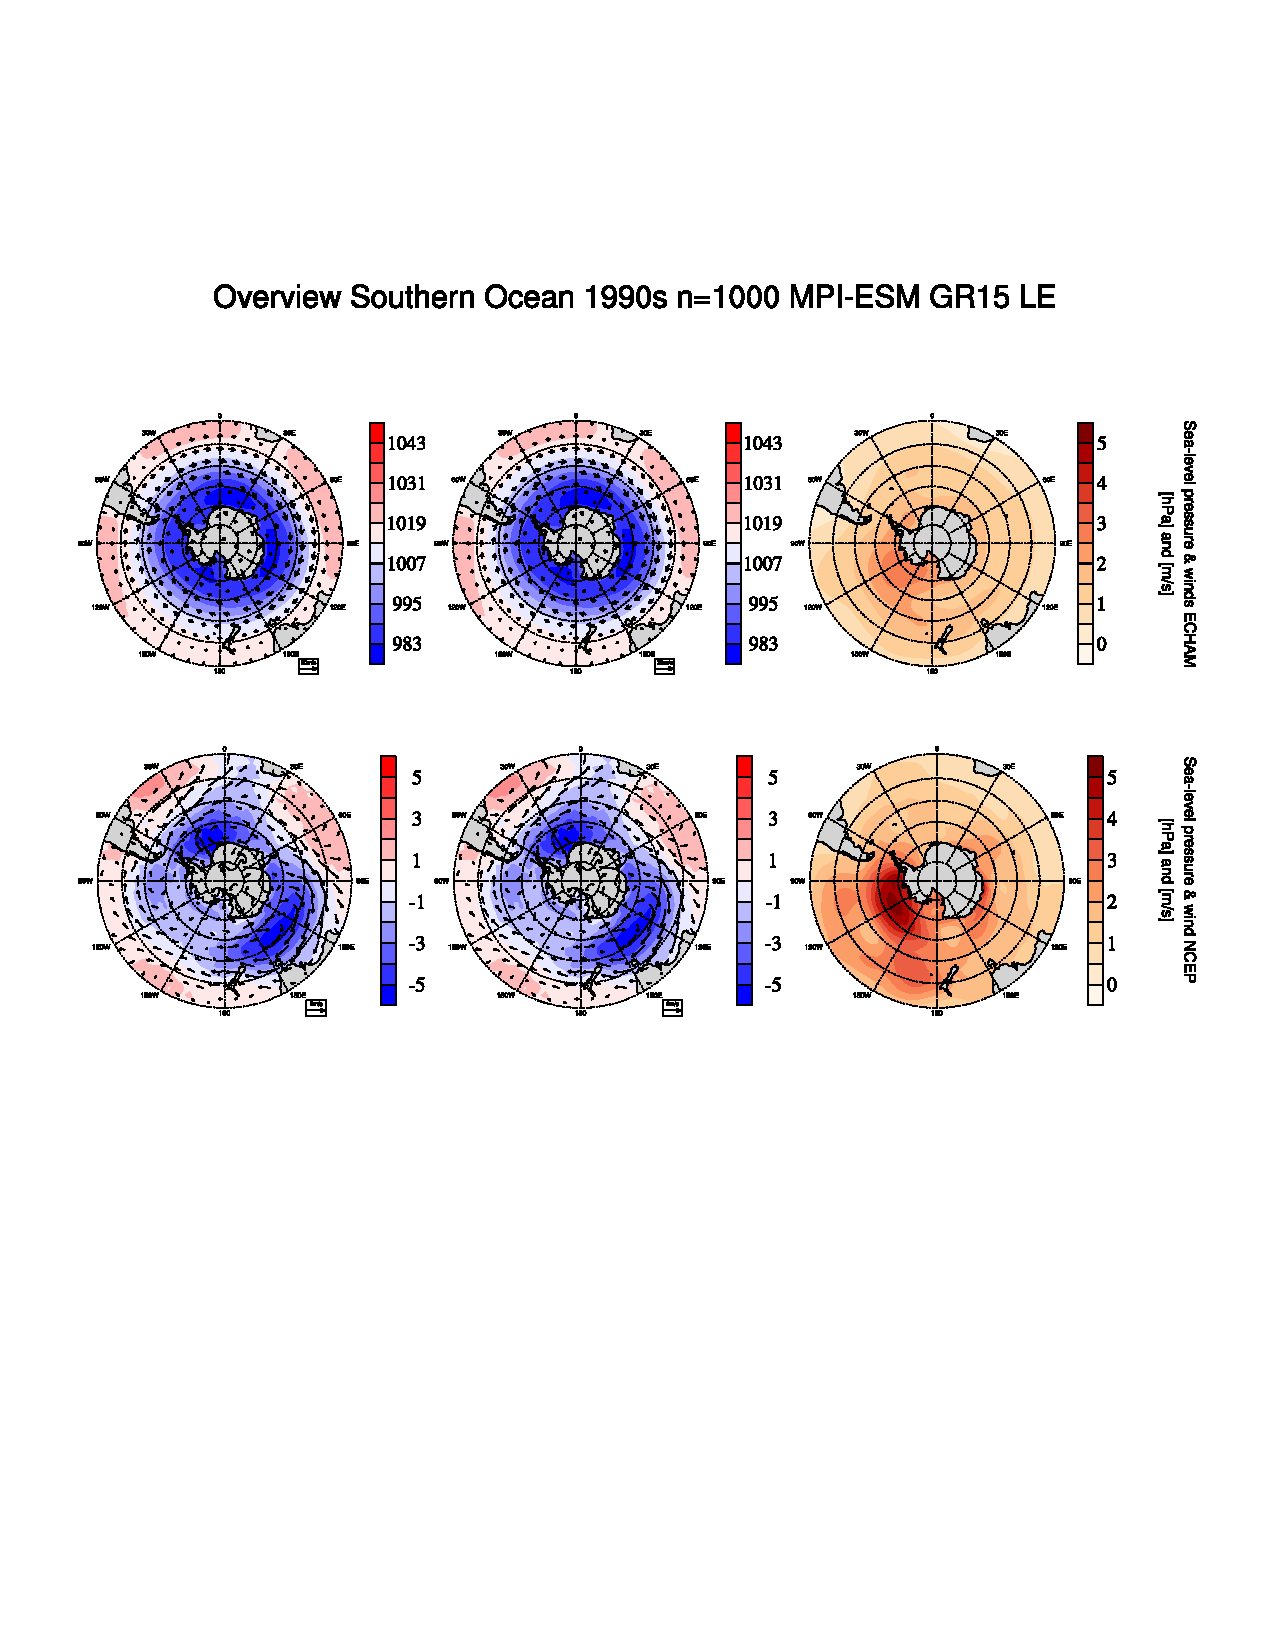
\includegraphics[scale=1.0,page=1,trim=13.4cm 16.5cm 2.5cm 7cm,clip]{Overview_SO_slp_ens_t1990s.pdf}} \\
       
        \subfloat[\acs{MPI-ESM}-\acs{NCEP} mean \acs{SLP} \text{[hPa/8yrs]}]
        {\label{fig:SO_winds_ensmean_ensstd-c}%
         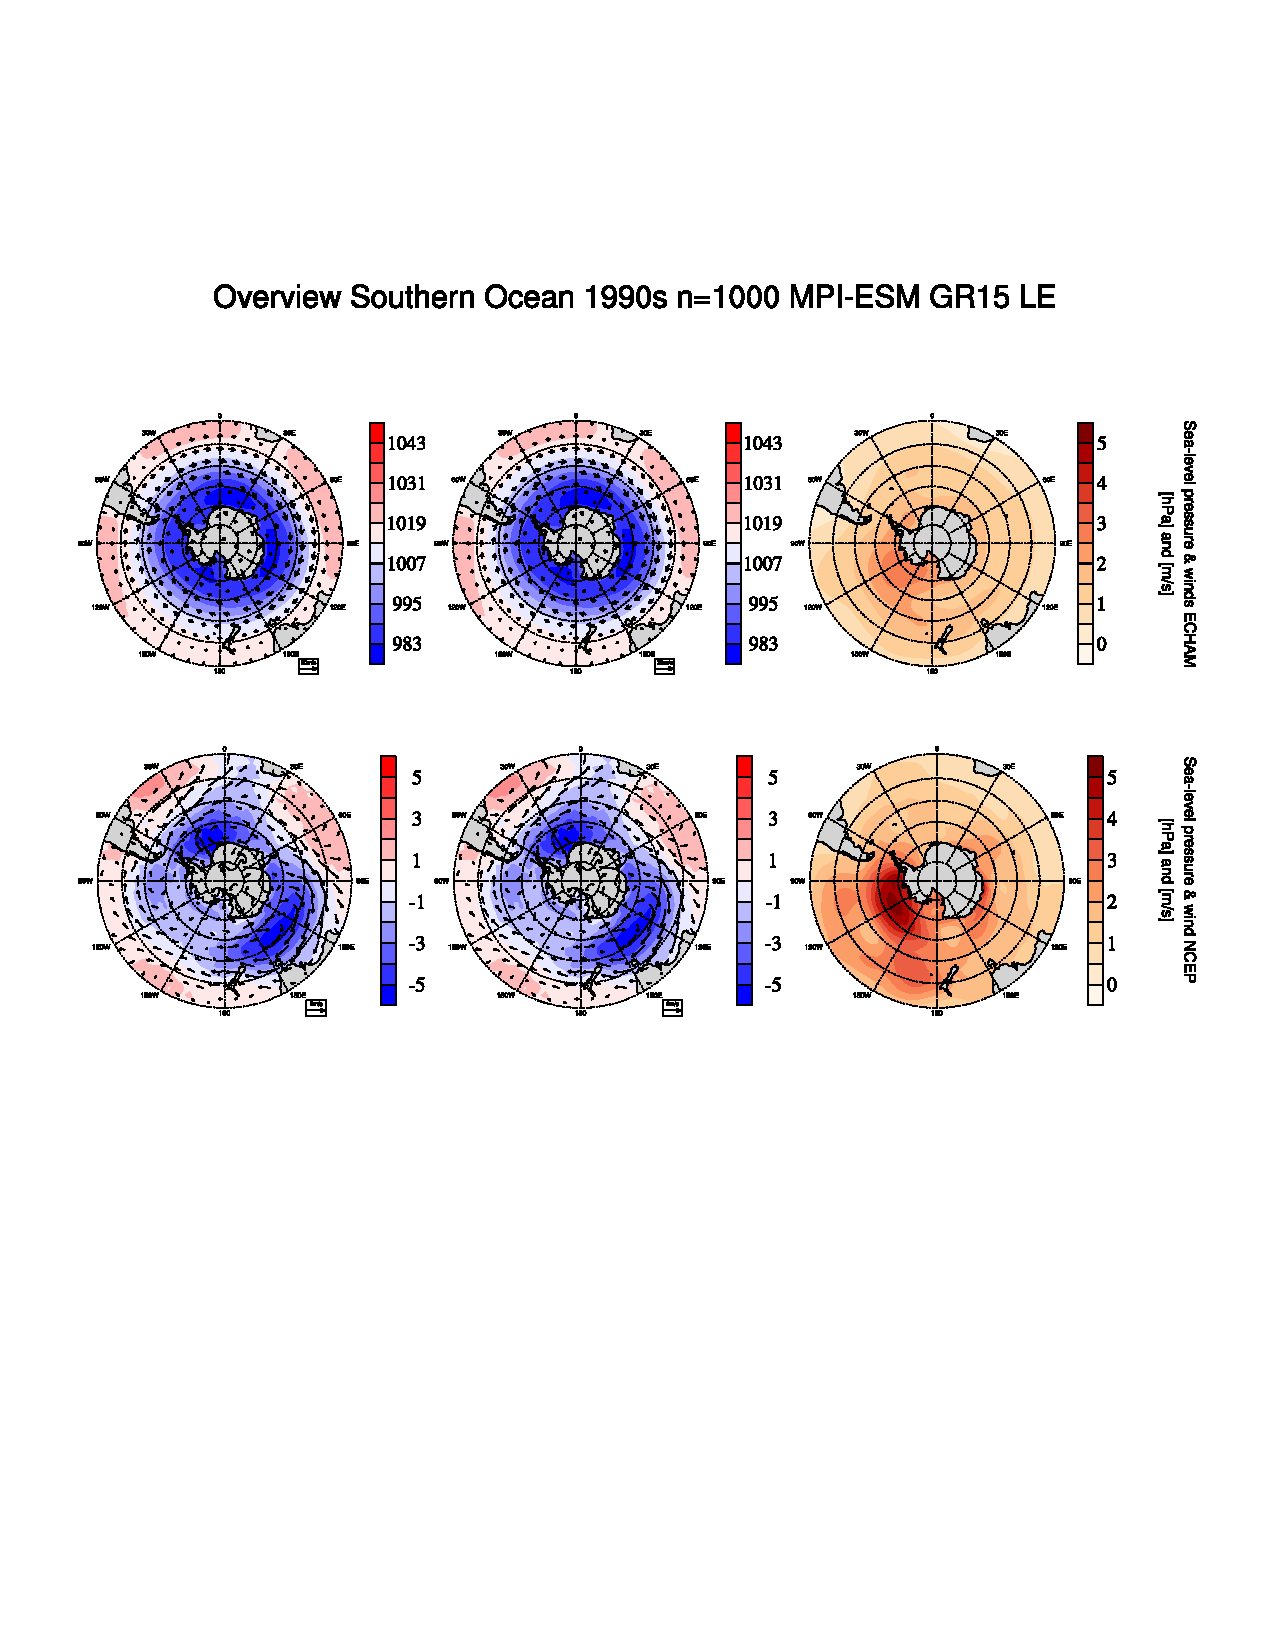
\includegraphics[scale=1.,page=1,trim=7.35cm 10.65cm 8.2cm 12.6cm,clip]{Overview_SO_slp_ens_t1990s.pdf}} 
        \subfloat[\acs{NCEP} \acs{SLP} $\sigma_{DIV}$ \text{[hPa/8yrs]}]
        {\label{fig:SO_winds_ensmean_ensstd-d}%
         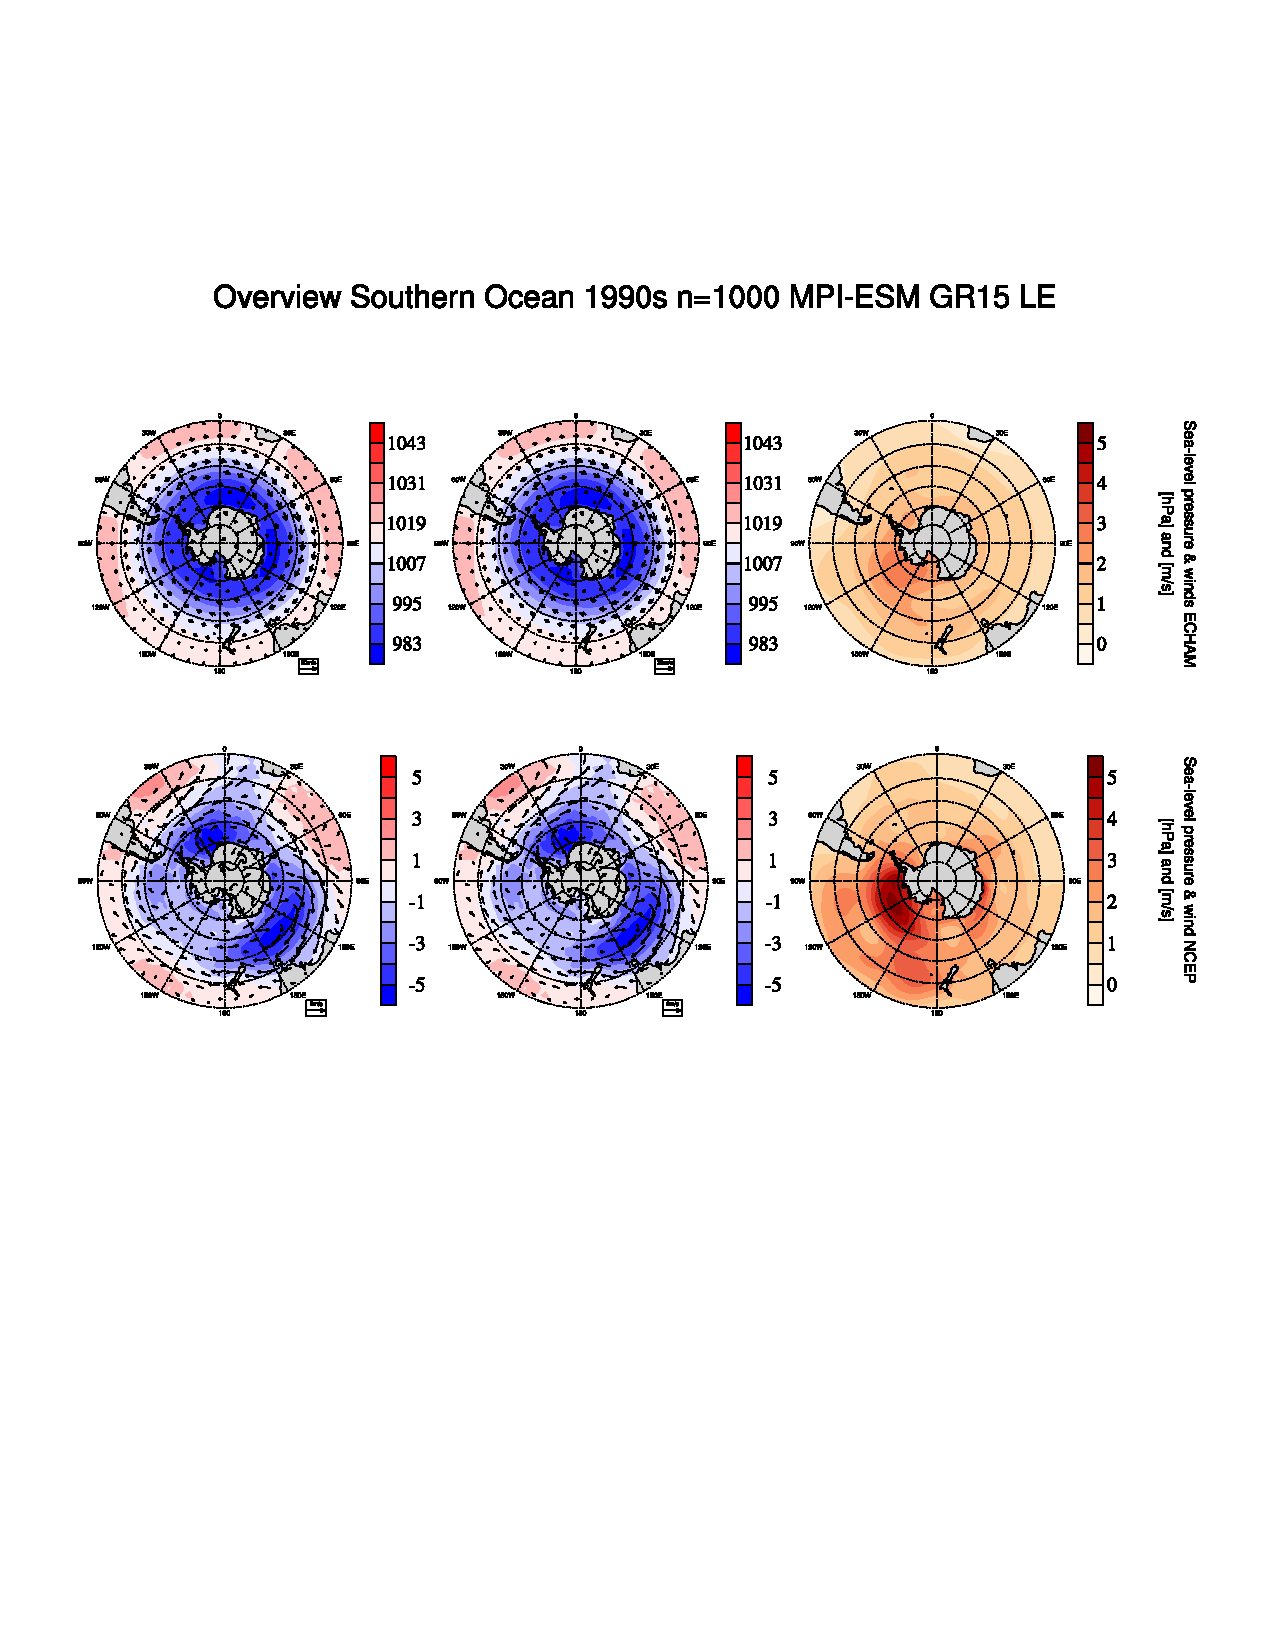
\includegraphics[scale=1.,page=1,trim=13.4cm 10.65cm 2.5cm 12.6cm,clip]{Overview_SO_slp_ens_t1990s.pdf}} 
        \caption{Spatial distribution of the Southern Ocean \acf{SLP} and wind vectors overlain as arrows: (a) \acs{MPI-ESM} ensemble mean climatology from 1980 to 2004 as forced signal, (b) ensemble decadal standard deviation as decadal internal variability $\sigma_{DIV}$; (c) difference between \acs{MPI-ESM} and reanalysis data from \acs{NCEP} reanalysis climatology \citep{Kalnay1996}, (d) decadal internal variability $\sigma_{DIV}$ from \acs{NCEP} reanalysis climatology.} \label{fig:SO_winds_ensmean_ensstd}
\end{figure}


%\paragraph{Temporal evolution of the mean state and internal variability}
The temporal evolution and internal variability of the annual \ac{SAM} index calculated according to \citep{Gong1999} (\autoref{sec:sam}) is shown in \autoref{fig:SO_winds_ensmean_ensstd}. Positive \acs{SAM} index values are associated with an anomalously low \acs{SLP} over Antarctica that result in a southward-shift and intensification of westerly winds. The \acs{MPI-ESM} ensemble mean has a positive trend as a consequence to anthropogenic CO$_2$ emissions and ozone depletion over Antarctica \citep{Thompson2011}.\newline


\begin{figure}[hbt]
        \myfloatalign
        \captionsetup[subfigure]{labelformat=empty,justification=centering}
        \subfloat[\acf{SAM} index \text{[1]}]
        {\includegraphics[scale=.48,angle=90,page=4,trim=4cm 1.2cm 4.5cm 2.5cm,clip]{co2flux_SO_timeseries_ymjm_35S_1980_2015_trend_8}} 
        \caption{Temporal evolution of the annual \acf{SAM} index according to \citep{Gong1999}. Grey lines show the 100 ensemble members; the black line the ensemble mean; the blue shading is the decadal internal variability $\sigma_{DIV}$; the red line reprensents the SAM during positive sea-air CO$_2$ flux trend; the blue line during the negative CO$_2$ flux trend; the green line shows the station-based \acs{SAM} from \cite{Marshall2003}.}\label{fig:evolution_SAM}
\end{figure}



%\paragraph{Temporal comparison to observational data} 
\acs{MPI-ESM LE} \ac{SAM} index lies in the range of the oberservational station-based \acs{SAM} index from \citep{Marshall2003}, although it follows a weaker trend in the ensemble mean.\newline

%\paragraph{Temporal evolution of extreme carbon trend members}
The positive CO$_2$ flux trend shows a positive trend in \acs{SAM}. Those strengthening winds increase upwelling (\autoref{sec:UOOC}), which brings over-saturated waters to the surface and hence leads to outgassing anomalies. This weakens the carbon sink and vice versa strengthens the carbon sink under the context of weakening westerly winds. The detailed response of primary production and advective transports under the context of changing winds is discussed in detail later in \autoref{ch:trends}.



\clearpage
\section{Biology}
\label{sec:biology}

%\paragraph{Spatial distribution in the mean state} %going from coast to north
%(fig. \autoref{fig:SOCS_ensmean_ensstd}a) 
The strong seasonal cycle in insulation and the sparseness of land topography leads to first-order zonally symmetric constraints for light and \ac{SST}. The high-latitude Southern Ocean is a so-called high nutrient low chlorophyll (HNLC) region, where light is the dominant limiting factor for the low biological production but nutrients are plenty \citep{Falkowski1998}. Summer sea-ice cover and sub-zero \acs{SST} values constrain plankton growth and is responsible for the tiny amount of primary production in the coastal areas as well as the Ross Sea and Weddell Sea. 

With decreasing latitude in the Southern Ocean, primary production increases along with increasing temperatures and light availability. Nutrients are upwelled by the upper-ocean overturning circulation and advected northwards by Ekman transport. This latitudinal increase of primary production peaks at 40-50$^\circ$S, where nutrients are abundant from upwelling and Ekman transport and higher temperatures and light availability foster phytoplankton growth rates. The mixing with warm subtropical waters off the Argentinian coast increases \acs{SST} and leads to a maximum primary production in the Southern Ocean \citep{Behrenfeld2014}. Downstream the Drake passage, the polar front with its cold waters extends more northward \citep{Orsi1995}. Along with lower nutrient concentrations due to increased precipitation from storms it explains the relatively low primary production in the Atlantic sector compared to other longitudinal counterparts. At the subtropical front decreasing nutrient concentrations limit primary production \citep{Behrenfeld2014} (\autoref{fig:SO_intpp_ensmean_ensstd}).\newline


%\paragraph{Spatial mean comparison to observational data}
To evaluate \acs{HAMOCC}'s ability to model the Southern Ocean, I do not compare modeled primary production to chlorophyll-a  concentration derived from satellite data, because satellite images are frequently  hidden by clouds. Instead, I compare the distributions of nitrate which is the limiting nutrient for biological production in this \acs{HAMOCC} version. %nitrate would be the limiting one
The distribution of nitrate shows a strong gradient in \acs{HAMOCC} as well as in the \ac{WOA} 2013  \citep{WOA2013} along the fronts from plentiful of nutrients in the high-latitudes to nutrient depletion in the subtropical gyres (\autoref{fig:SO_comp_nitrate}). In higher latitudes \acs{HAMOCC} underestimates the phosphate concentration by 25\%. These lower nutrient concentrations can be a sign of more nutrient consumption at higher primary production or be the reason for lower primary production. The distribution of another important nutrient phosphate shows a similar spatial pattern (\autoref{fig:SOCS_comp_phosph}).\newline

%\paragraph{Spatial distribution of internal variability} 
Internal decadal variability in vertically integrated primary production in the Southern Ocean is higher in high productivity areas (\autoref{fig:SO_intpp_ensmean_ensstd-b}). The whole region at 45-60$^\circ$S, especially in the Indian sector, shows a enormously high decadal internal variability $\sigma_{DIV}$ relative to the ensemble mean state. Internal variability in the Southern Hemisphere is mostly driven by westerly winds. The explicit effect of those on \acs{HAMOCC} is discussed in \autoref{ch:trends}.\newline


\begin{figure}[bth]
        \myfloatalign
        \subfloat[\acs{MPI-ESM} \acs{INTPP} ensemble mean \text{      }  \text{      } \text{[kgC m$^{-2}$ yr$^{-1}$]}]
        {\label{fig:SO_intpp_ensmean_ensstd-a}%
       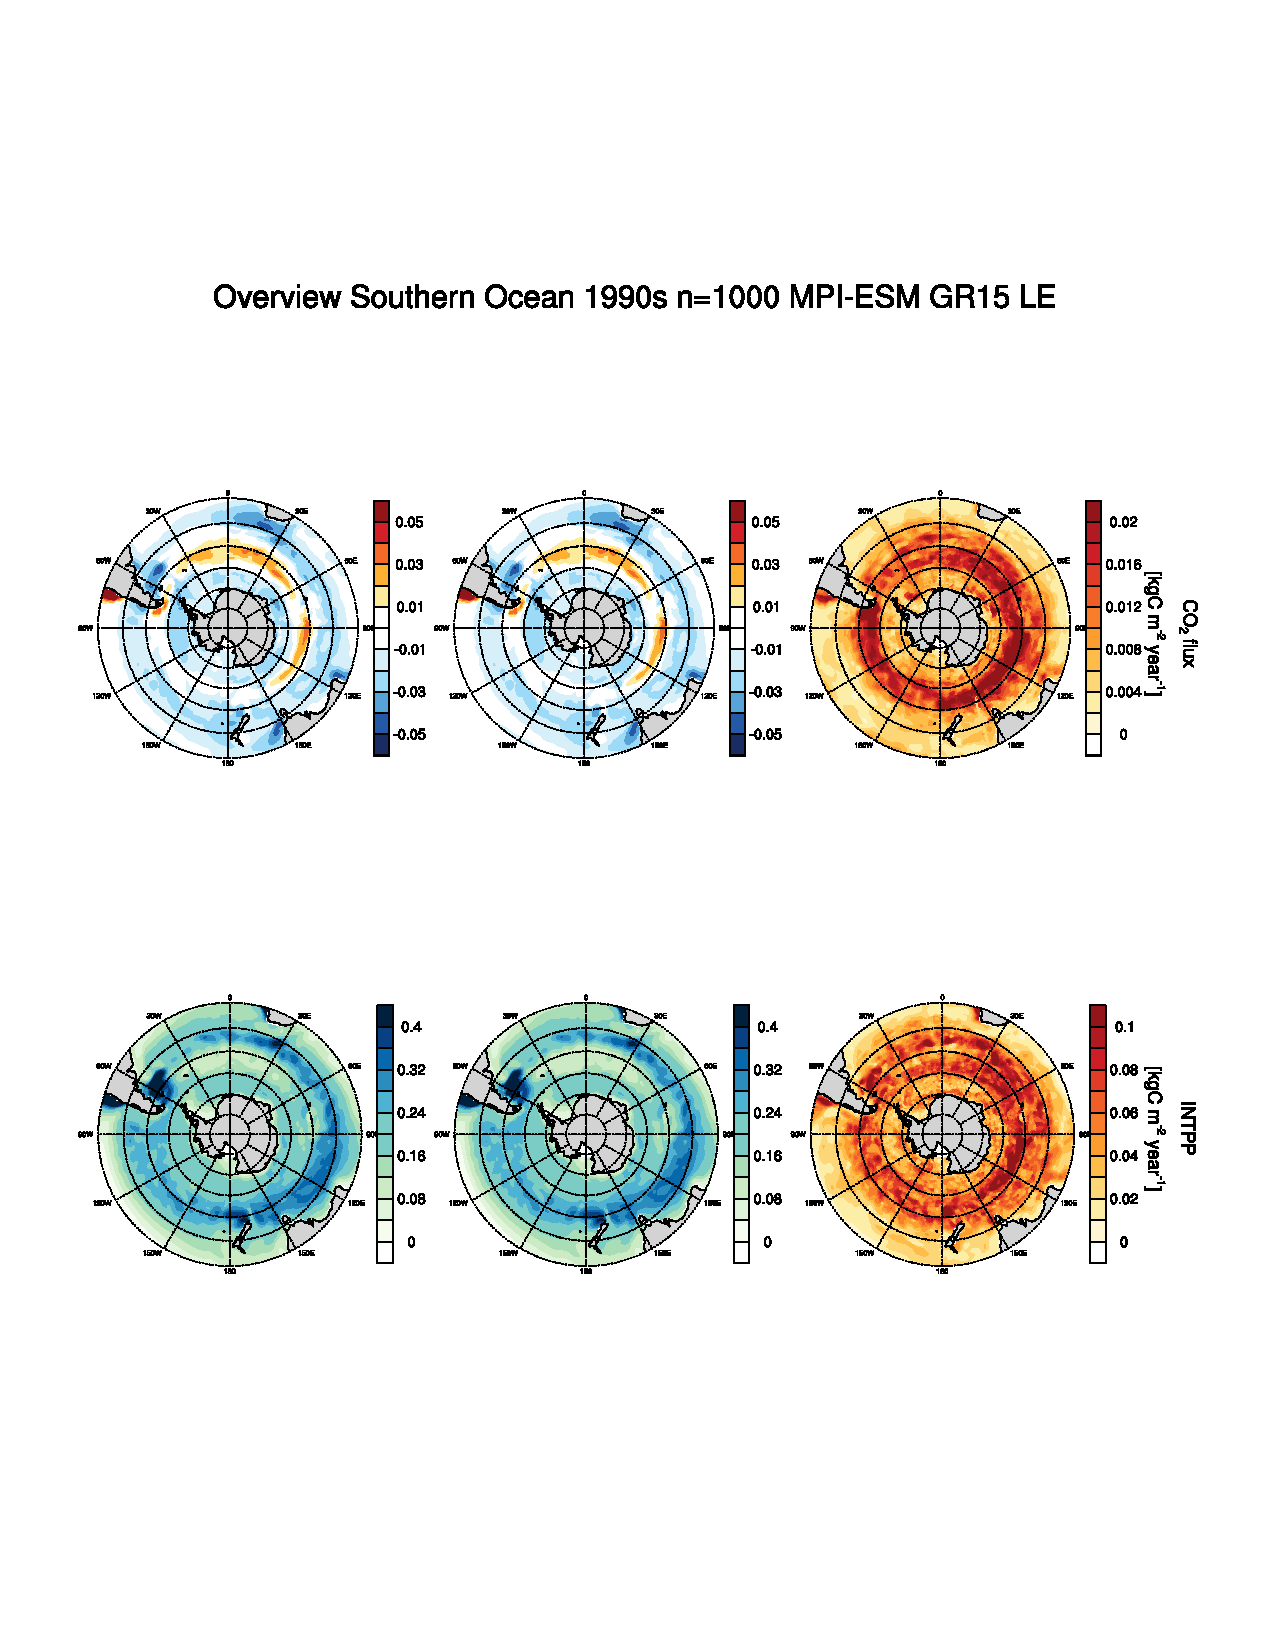
\includegraphics[scale=.97,trim=7.25cm 6.3cm 8.2cm 16.8cm,clip]{Overview_SO_co2flux_intpp_ens_t1990s.pdf}} %\quad
        \subfloat[\acs{MPI-ESM} \acs{INTPP} $\sigma_{DIV}$ \text{      }  \text{      } \text{      }  \text{      } \text{[kgC m$^{-2}$ yr$^{-1}$]}]
        {\label{fig:SO_intpp_ensmean_ensstd-b}%
         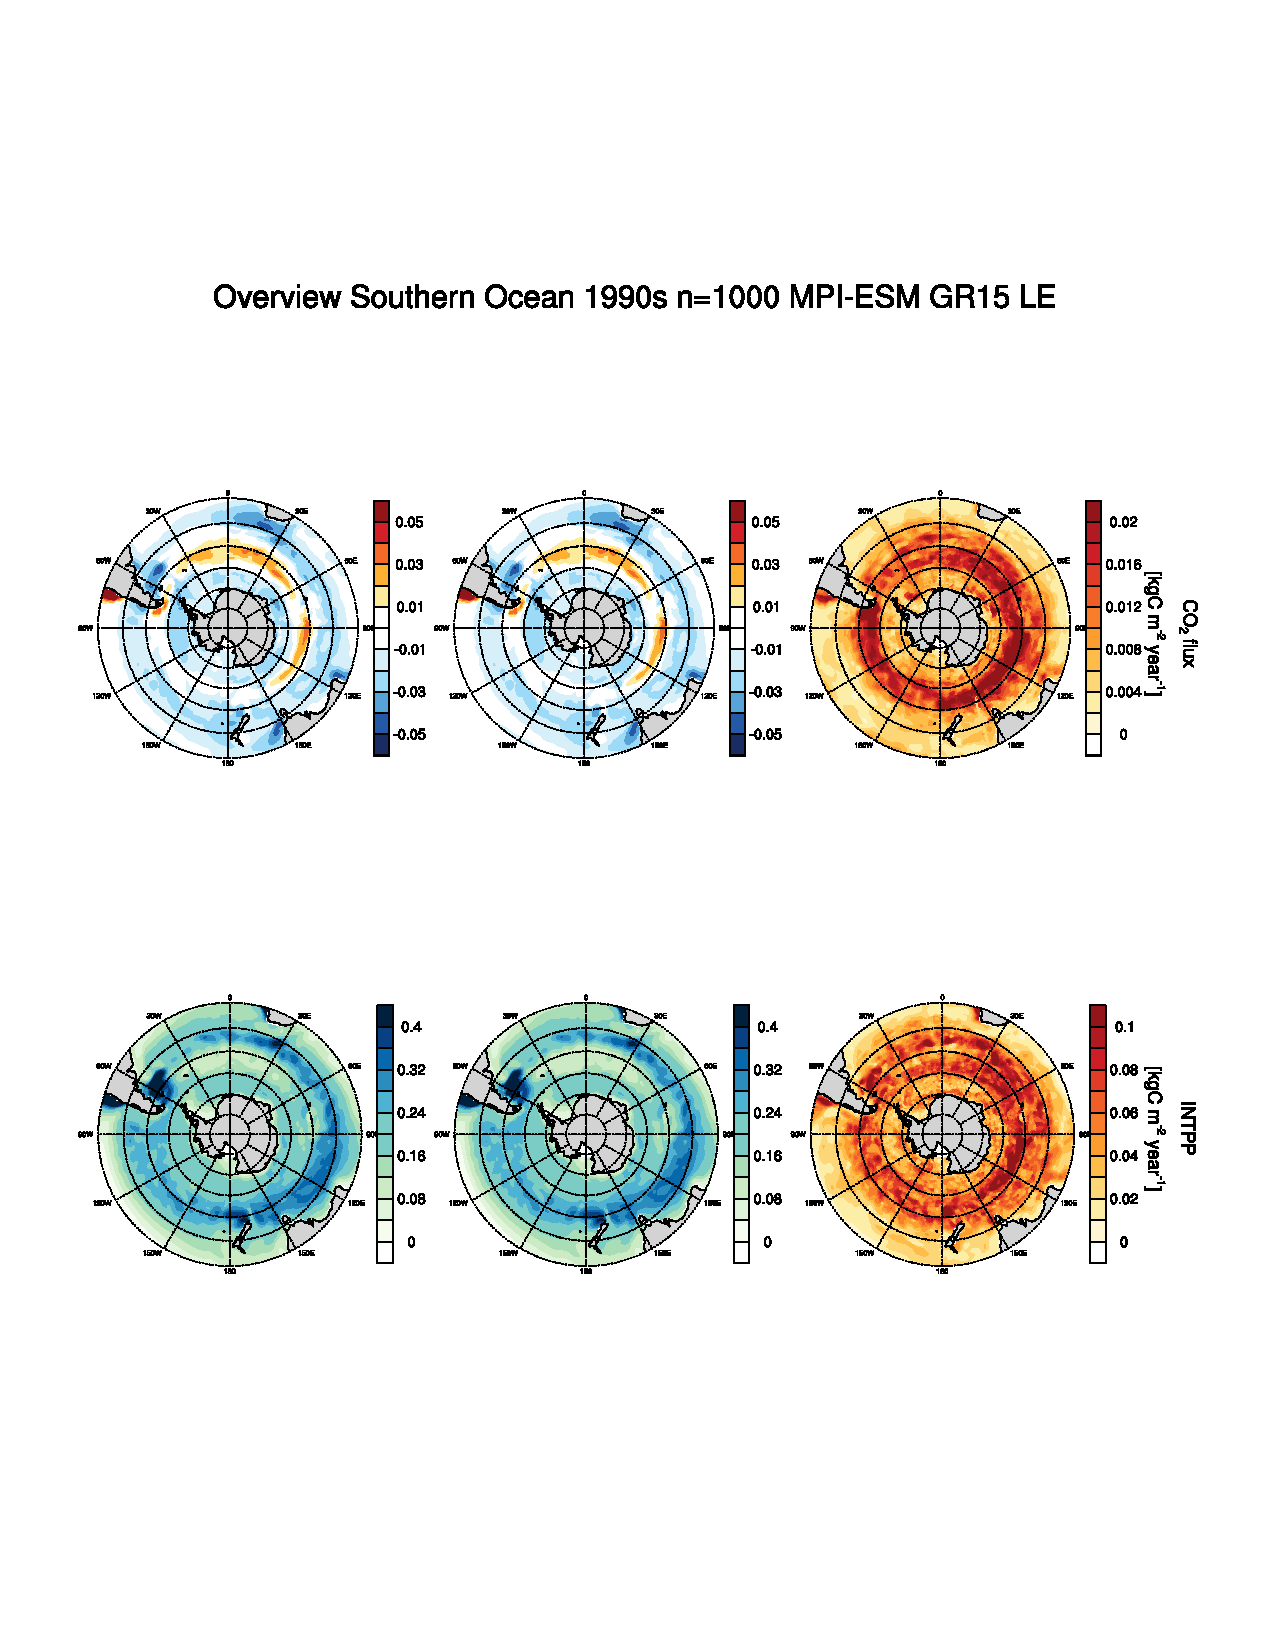
\includegraphics[scale=.97,trim=13.3cm 6.3cm 2.25cm 16.8cm,clip]{Overview_SO_co2flux_intpp_ens_t1990s.pdf}} \\
        \caption{Spatial distribution of the vertically integrated primary production in the Southern Ocean: (a) climatological \acs{MPI-ESM} ensemble mean from 1980 to 2004 as forced signal and (b) ensemble decadal anomaly standard deviation as decadal internal variability $\sigma_{DIV}$.} \label{fig:SO_intpp_ensmean_ensstd}
\end{figure}

\begin{figure}[bth]
        \myfloatalign
        \subfloat[\acs{MPI-ESM} surface nitrate ensemble mean \text{      }  \text{      } \text{[mmol N m$^{-3}$]}]
        {\label{fig:SO_comp_nitrate-a}%
       \includegraphics[scale=.66,page=3,trim=1.3cm 13.3cm 12.1cm 6.5cm,clip]{Overview_SO_nutrient_comparison.pdf}} %\quad
        \subfloat[\acs{WOA} surface nitrate mean \text{      }  \text{      } \text{      }  \text{      } \text{      }  \text{      }\text{[mmol N m$^{-3}$]}]
        {\label{fig:SO_comp_nitrate-b}%
         \includegraphics[scale=.66,page=3,trim=9.4cm 13.3cm 2.1cm 6.5cm,clip]{Overview_SO_nutrient_comparison.pdf}} \\
        \caption{Spatial distribution of surface nitrate in the Southern Ocean: (a) \acs{MPI-ESM} ensemble mean climatology, (b) \acf{WOA} climatology data \citep{WOA2013}.} \label{fig:SO_comp_nitrate}
\end{figure}

%\paragraph{Temporal evolution of the mean state and internal variability}
Regarding the temporal evolution in the Southern Ocean, primary production is not subject to a strong forced trend in the historical period but varies internally (\autoref{fig:evolution_southern_ocean_intpp}). The weak decreasing trend might be the first sign of increased stratification due to sea-surface warming, which in turn inhibits the mixing of nutrients. But the long-term consequences for primary production is subject to ongoing research and debate \citep{Bopp2013,Taucher2011,Lozier2011,Kessler2016,Krumhardt2017,Deppeler2017}. The decadal internal variability $\sigma_{DIV}$ is 0.5 PgC/yr/decade.

\begin{figure}[bth]
        \myfloatalign
	    \captionsetup[subfigure]{labelformat=empty,justification=centering}        
        \subfloat[\acf{INTPP} \text{[PgC/yr]}]
        {\includegraphics[scale=.48,angle=90,page=3,trim=4cm 1.2cm 4.5cm 2.5cm,clip]{co2flux_SO_timeseries_ymjm_35S_1980_2015_trend_8}} 
		\caption{Temporal evolution of the \acf{INTPP} in the Southern Ocean south of 35$^\circ$S. Grey lines show the 100 ensemble members, the black line the ensemble mean, the blue shading is the decadal internal variability $\sigma_{DIV}$, the red line shows \acs{INTPP} during the positive CO$_2$ flux trend, the blue line during the negative CO$_2$ flux trend.}	\label{fig:evolution_southern_ocean_intpp}
\end{figure}

The absolute amount of primary production exceeds CO$_2$ flux by a factor of $\sim$20. The spatial distribution of export flux at $90m$, which is the particulate organic matter that sinks below the euphotic zone, is the same as for primary production. As a lower vertical boundary for a upper-ocean budget, export flux is of similar magnitude as CO$_2$ flux and thus comparable (\autoref{ch:pCO2separation}).\newline

%\paragraph{Temporal evolution of extreme CO$_2$ flux trends}
The negative CO$_2$ flux trend has a positive trend in primary production, because primary production lowers surface \acs{DIC}, pCO$_{2\text{,ocean}}$ and hence reduces CO$_2$ uptake by the ocean; and vice versa negative trends in primary production lead to positive CO$_2$ flux trends.\newline 

%\paragraph{HAMOCC Southern Ocean performance}
\acs{MPI-ESM} is able to model the general features of the Southern Ocean, such as the characteristics of a high nutrient low chlorophyll region \citep{Bopp2013}. But compared to other models and observational data, the seasonal cycle of phytoplankton blooms is amplified and too early in the Southern Ocean \citep{Bopp2013,Nevison2015,Nevison2016}. The reason of this is under current debate in the MPI biogeochemistry research group. It could involve that the Southern Ocean in \acs{MPI-ESM LE} runs is not iron-limited but while changing the dust input fields and the iron cycling constants lead to an iron-limited Southern Ocean the amplified seasonality is still present [private Communication, Irene Stemmler (MPI, Hamburg)]. Also a look into the grazing of zooplankton and its variable formulation might lead to a more realistic primary production seasonality. Furthermore, the atmospheric bias in westerly winds and the Southern Ocean warm bias \citep{Jungclaus2013} hinders sea-ice to propagate more extensively. A proper representation of Antarctic sea-ice would come along with a cooler, more stratified Southern Ocean which modulates primary production. But the amplified seasonality also occurs in the norwegian \acs{ESM} NorESM which uses \acs{HAMOCC} in a different ocean model, so revisiting seasonality in the high-latitude oceans remains a challenge in \acs{HAMOCC}.

Additionally, the longest standing data records, which are on the northern hemisphere in Iceland \citep{Six1996}, are used for the tuning of free model parameters. Historically, the Southern Ocean has never been in the focus of \acs{HAMOCC}. 









\clearpage

\section{Upper-Ocean Overturning Circulation}
\label{sec:UOOC}

%\paragraph{Spatial distribution in the mean state and internal variability}
The Southern Ocean upper-ocean overturning circulation is driven by the divergence at 40-60$^\circ$S corresponding to strong westerly winds (\autoref{fig:UOOC_mean-a}). 
The isopyncals, which separate water masses, orient themselves at values from \cite{Sallee2013a}, but are shifted to fit to typical depths, which is a common feature in water mass comparison as models have different density biases \citep{Sallee2013a}. 
In the high latitudes south of 50$^\circ$S Ekman pumping brings \ac{CDW} from the ocean interior to the surface. At the surface these waters are transported to the north. At lower latitudes, the surface waters warm and evaporation increases, so relatively cold and low salinity waters known as \ac{AAIW} slide below warmer and more saline \ac{SAMW} to extend northwards at intermediate depth. This process is called downwelling or Ekman subduction.  

The strong upper-ocean overturning circulation in the Southern Hemisphere features upwelling south of 50$^\circ$S, northward transport at 40-60$^\circ$S and downwelling at 30-40$^\circ$S and is known as the Deacon cell \citep{Doeoes1993,Speer2000}. The upper-ocean overturning circulation is driven by the strength and positions of westerly winds. Upwelling steepens and downwelling straightens the isopycnals along which the water masses flow \citep{Marshall2012}. The internal variability in the horizontal processes at intermediate depth is lower than at the surface because the influence of winds decays with depth. The decadal internal variability $\sigma_{DIV}$ of vertical Ekman pumping and subduction is of similar magnitude at 200m and 1000m (\autoref{fig:UOOC_mean}).\newline

%\paragraph{Comparison to observational data}
{\color{RoyalBlue}Fig.} \ref{fig:UOOC_mean-a} is similar to \cite[fig. 1]{DeVries2017}, which uses observational data in an inverse model to demonstrate changes in upper-ocean overturning circulation. Due to different vertical velocity regimes I choose different boundaries for the transport which prevents me from quantitative comparisons. Nevertheless, data of \cite[fig. 1]{DeVries2017} show the main characteristics of the Deacon cell and water transport of comparable magnitude as in \acs{MPI-ESM LE}. \newline



\begin{figure}[h!]
        \myfloatalign
        \subfloat[\acs{MPI-ESM} advective water transport \text{[Sv]}]
        {\label{fig:UOOC_mean-a}%
       \includegraphics[scale=0.45,page=4,trim=1.4cm 1.7cm 0cm 4.6cm,clip]{UOOC}} \quad
        \subfloat[\acs{MPI-ESM} advective carbon transport \text{[PgC/yr]}]
        {\label{fig:UOOC_mean-b}%
         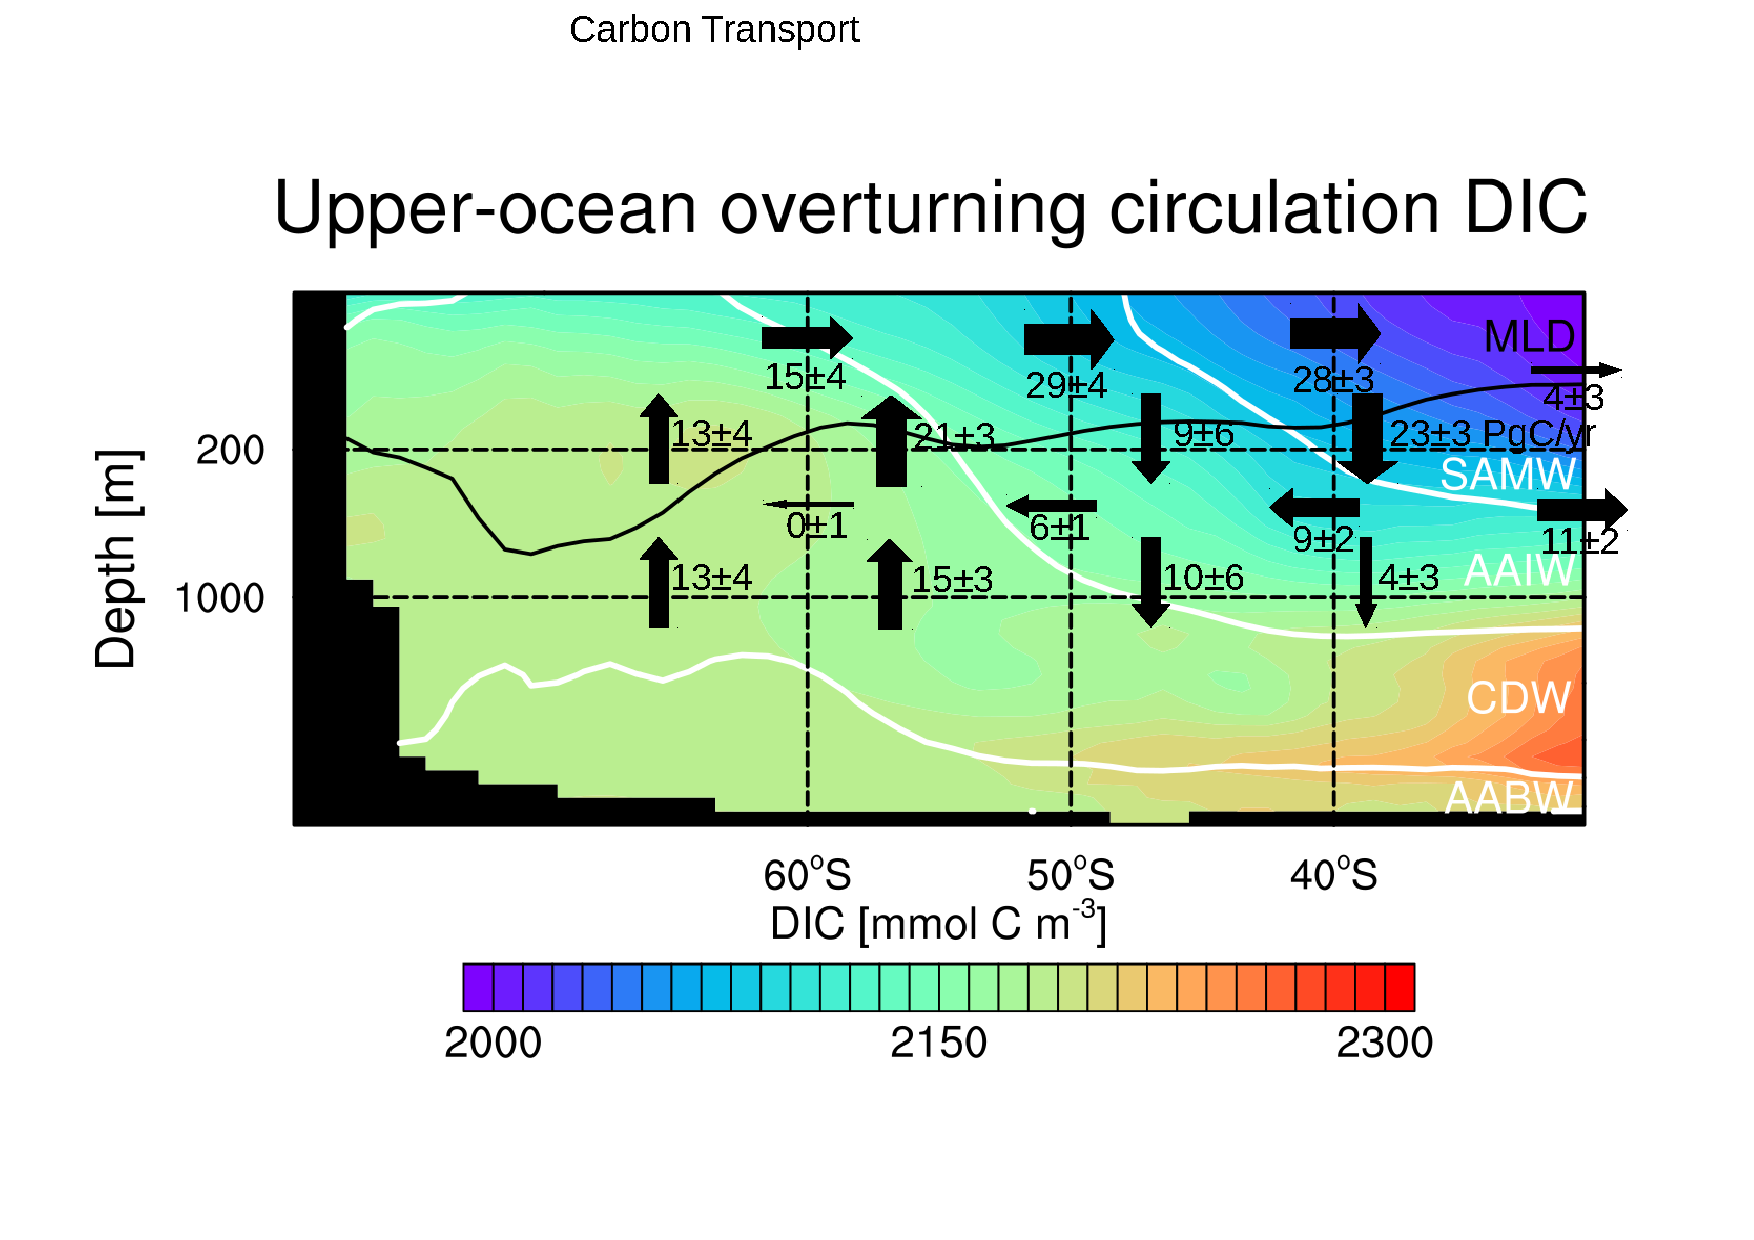
\includegraphics[scale=0.45,page=1,trim=.8cm 1.7cm 0cm 4.6cm,clip]{UOOC}} \\
        \caption{Zonally averaged transect of the Southern Ocean and the upper-ocean overturning circulation; black arrows show yearly mean advective transports and decadal internal variability $\sigma_{DIV}$ of (a) water in Sv and (b) carbon in PgC/yr; white lines are isopyncals separating \ac{SAMW} at potential density $\rho_{\theta\text{}}=1026.5$ kg m$^{-3}$ from \ac{AAIW}, at $\rho_{\theta\text{}}=1027.2$ kg m$^{-3}$ from \ac{CDW}, at $\rho_{\theta\text{}}=1027.7$ kg m$^{-3}$ from \ac{AABW}; the black line is the \ac{MLD}; the colored contours show the distribution of concentration in \acs{DIC}.} \label{fig:UOOC_mean}
\end{figure}



%\paragraph{Link to the carbon cycle}
How does the upper-ocean overturning circulation relate to the carbon cycle? The concentration of \acs{DIC} in general increases with depth due to the biological pump and remineralization at depth. This is most clearly seen in the subtropics and blurred by processes of mixing at higher latitudes (\autoref{fig:UOOC_mean}). Still, upwelled waters from the deep oceans have a high pCO$_2$ potential at which they would equilibrate when lifted to the surface, so the upwelling super-saturated waters in high latitude waters drives CO$_2$ outgassing and downwelling takes CO$_2$ equilibrated waters into the deeper ocean (\autoref{fig:UOOC_mean-b}) \citep{Morrison2015}.\newline 

%\paragraph{Temporal evolution of the mean state and internal variability} I would need to construct an index

%\paragraph{Trends of extreme carbon trend members}
During the positive CO$_2$ flux trend upper-ocean overturning circulation intensifies. This means enhanced upwelling, which weakens the carbon sink (\autoref{fig:UOOC_neg}) and vice versa strengthens the carbon sink for weaker upper-ocean overturning circulation (\autoref{fig:UOOC_pos}). %[I could to construct an index to have a similar figure as before, but dont know whether what would be really nessessary for the story.]

%\paragraph{Temporal comparison to observational data}  no data; a bit compared to DeVries


%\paragraph{MPI-OM Southern Ocean performance evaluation}  
The global performance of \acs{MPIOM} is discussed in detail in \cite{Jungclaus2013}. The Southern Ocean \acs{SST} warm bias is attributed to an overestimation of downward shortwave radiation into the polar regions \citep{Stevens2013} and causes the underestimation of sea-ice coverage. Additionally, the water-column stability is too low which allows open-ocean convection in the Ross and Weddell Sea and deeper than observed winter mixing. %Heat from the relatively warm circumpolar deep waters warms the subsurface waters \citep{Stoessel2015}. 
Additional freshwater input from melting glaciers distributed by icebergs improves the water-column stability, increases sea-ice and prevents open-ocean convection. A similar effect has the coupling to a higher resolved atmosphere due to additional freshwater input from circulation pattern changes \citep{Stoessel2015}. 

%\subparagraph{Water mass circulation}
The model quality of overturning circulation in the Southern Ocean is analyzed by \cite{Sallee2013a}. \acs{MPI-ESM} realistically simulates subtropical water temperature and Sub-Antarctic Mode Water in general. But the overturning cell is much weaker than in other models.

%\subparagraph{ZMLD comparison} 
The \ac{MLD} is an important measure to assess how climate models represent the Southern Ocean. \acs{MLD} in \acs{MPI-ESM} is overestimated compared to observational data from \acs{NOAA} Atlas \citep{Monterey1997} in the locations of the \ac{ACC} and the Ross and Weddell Sea (\autoref{fig:SO_comp_zmld}) as well as in the zonal average (\autoref{fig:UOOC_mean}). In the Ross and Weddell Sea the \acs{MLD} deepens to few kilometers depth via open-ocean convection \citep{Stoessel2015}, which often appears in climate models but rarely seen in observations \citep{Heuze2013,deLavergne2014}. The weak stratification explains why \acs{MPI-ESM} overestimates \acs{MLD}; especially in winter \citep{Sallee2013}.



\begin{figure}[bth]
        \myfloatalign
        \subfloat[\acs{MPI-ESM} \acs{MLD} ensemble mean \text{[m]}]
        {\label{fig:SO_comp_zmld-a}%
       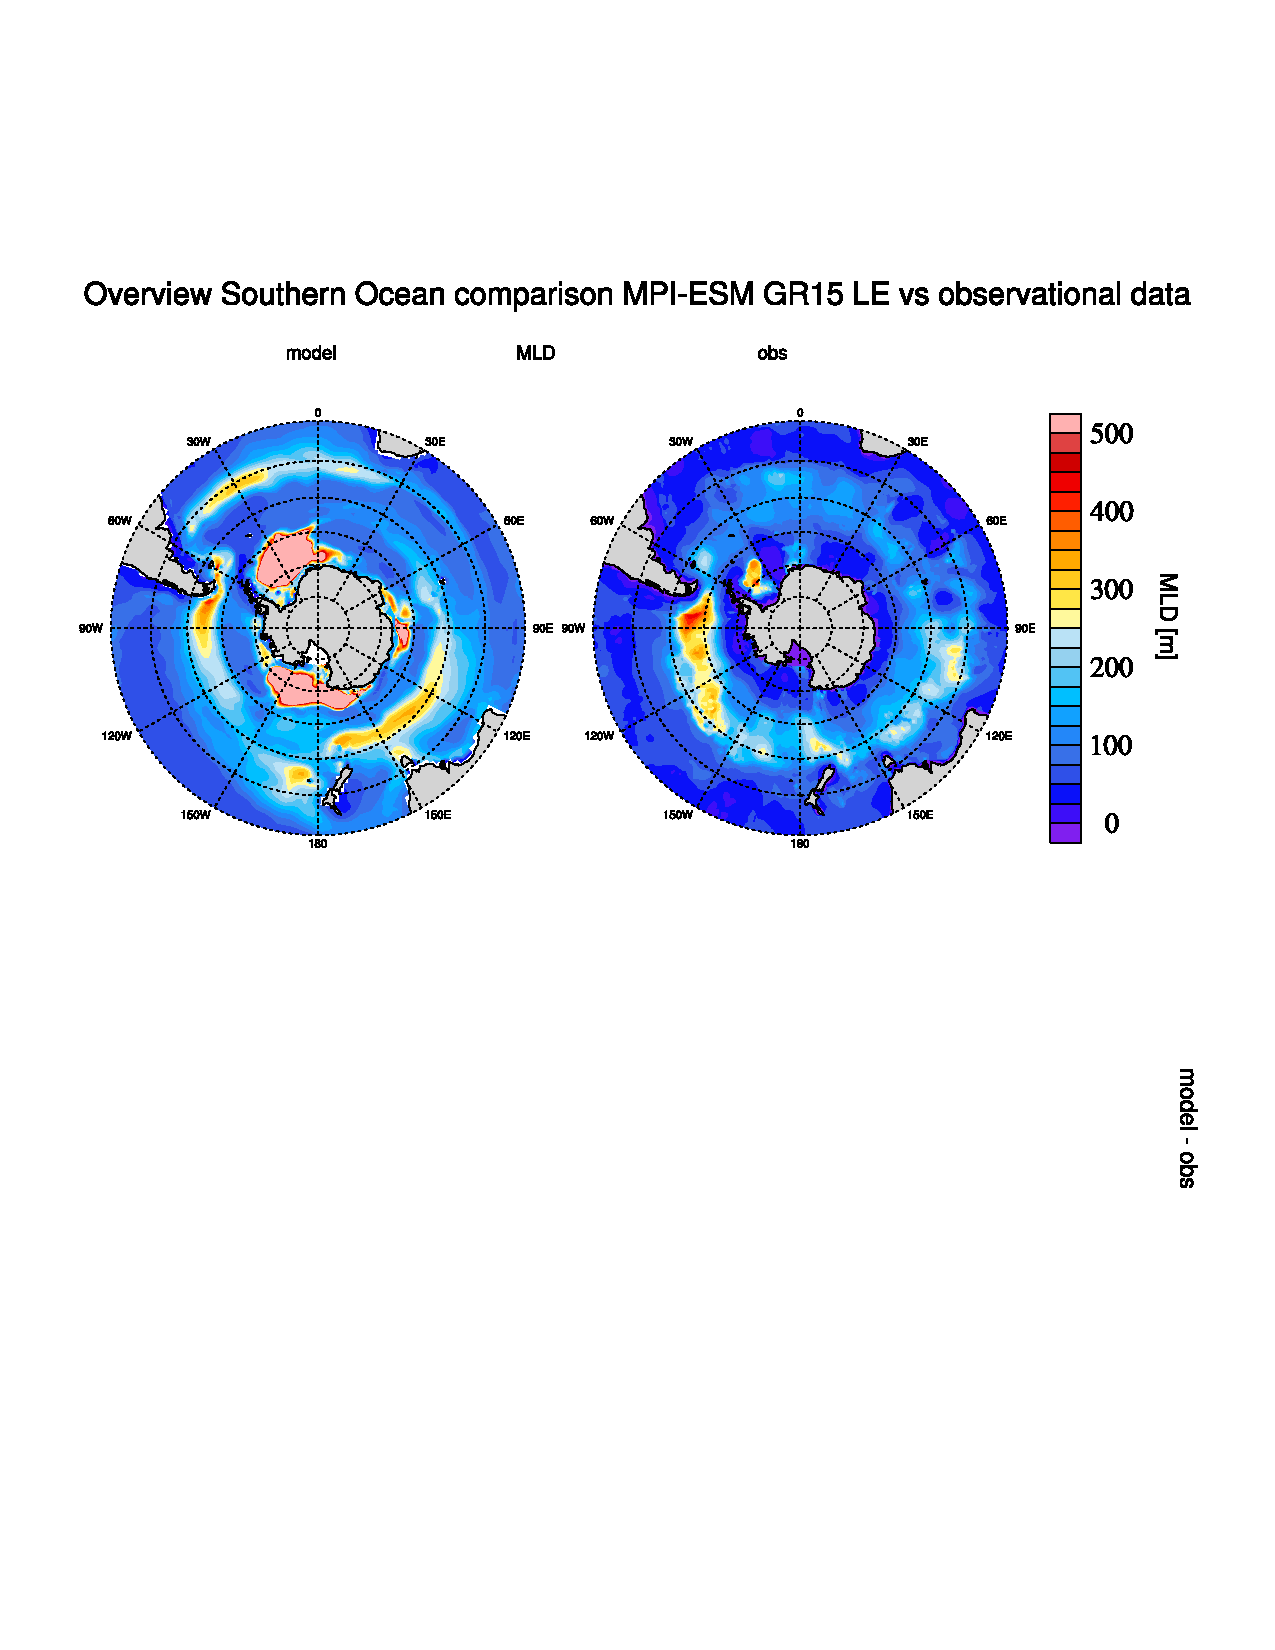
\includegraphics[scale=.66,page=1,trim=1.25cm 13.3cm 12.08cm 6.5cm,clip]{Overview_SO_MPIOM_comparison.pdf}} %\quad
        \subfloat[\acs{NOAA} \acs{MLD} Atlas mean \text{[m]}]
        {\label{fig:SO_comp_zmld-b}%
         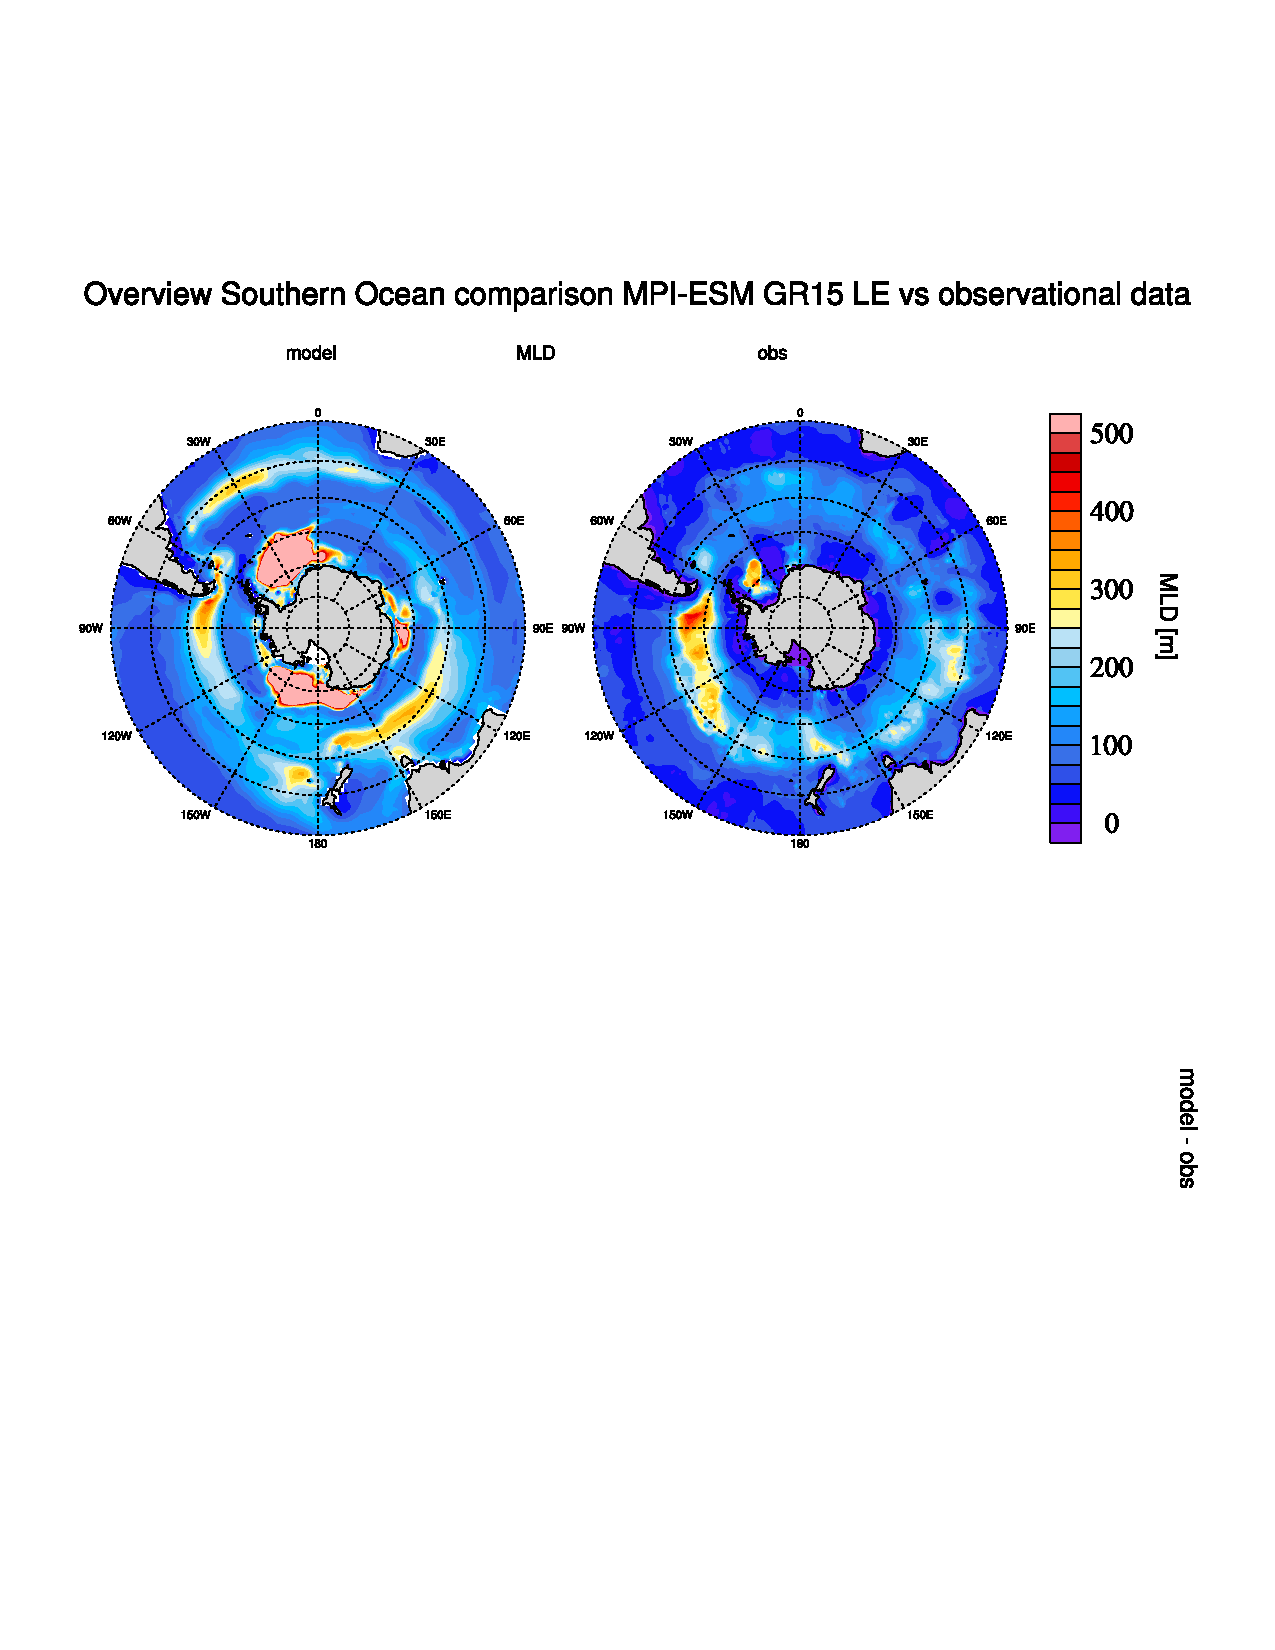
\includegraphics[scale=.66,page=1,trim=9.4cm 13.3cm 2.1cm 6.5cm,clip]{Overview_SO_MPIOM_comparison.pdf}} \\
        \caption{Spatial distribution of \acf{MLD} in the Southern Ocean: (a) \acs{MPI-ESM} ensemble mean climatology, (b) \acs{NOAA} Atlas climatology \citep{Monterey1997}.} \label{fig:SO_comp_zmld}
\end{figure}
